\documentclass[12pt, a4paper]{article}

\usepackage[brazil]{babel}
\usepackage[utf8]{inputenc}
\usepackage{amsmath}
\usepackage{amssymb}
\usepackage{amsthm}
\usepackage{float}
\usepackage{enumerate}
\usepackage{graphicx}
\usepackage{euler}
\usepackage[pdfstartview=FitH]{hyperref}
\usepackage{caption}
\usepackage{subcaption}

% http://ctan.org/pkg/pifont (for checkmarks)
\usepackage{pifont}                 
\newcommand{\cmark}{\ding{51}}
\newcommand{\xmark}{\ding{55}}

\newtheorem{teor}{Teorema}[section]
\newtheorem{lema}[teor]{Lema}
\newtheorem{prop}[teor]{Proposição}
\newtheorem{coro}[teor]{Corolário}
\theoremstyle{definition}
\newtheorem{defi}[teor]{Definição}
\newtheorem{exem}[teor]{Exemplo}
\newtheorem{exer}{Exercício}

\title{Grafos: introdução.}
\author{Daniel M. Martin}
\date{2018.Q3}

\begin{document}
\maketitle

\section{Definições básicas}

$\rhd$ História das pontes de Königsberg.

\subsection{Grafo}

%Para um conjunto~$V$ e um inteiro $k \geq 0$, denote por ${V \choose k}$ a família de todos os $k$-subconjuntos de~$V$. Mais formalmente, definimos 
%\[ {V \choose k} = \{W \subseteq V \colon |W| = k\}. \]
%Por exemplo, se $V = \{1,2,3,4\}$, então 
%\[ {V \choose 2} = \big\{\{1,2\},\{1,3\},\{1,4\},\{2,3\},\{2,4\},\{3,4\}\big\}.\]
\noindent Um \emph{grafo} é um par ordenado $(V,E)$, onde $V$ é um conjunto qualquer e $E$ é um subconjunto de pares não ordenados de $V$. %, ou seja, $E$ satisfaz
%\[ E \subseteq {V \choose 2}. \]
Os elementos de $V$ são chamados de \emph{vértices} e os elementos de $E$ são chamados de \emph{arestas}. 

\begin{exem}
\label{exem:umgrafo}
O par ordenado $\big(\{1,2,3,4,5\}, \big\{\{1,2\}, \{1,4\}, \{2, 4\}, \{3,5\}\big\}\big)$ é um exemplo de grafo que tem os números inteiros de~$1$ a $5$ como vértices e que possui~$4$ arestas. 
\end{exem}

O nome grafo vem do fato de que esses objetos podem ser representados graficamente por diagramas. Vértices do grafo correspondem a pontos do diagrama e arestas do grafo correspondem a linhas que ligam esses pontos.

\begin{exem}
O grafo do Exemplo~\ref{exem:umgrafo} pode ser representado de diversos modos em um diagrama. A Figura~\ref{fig:umgrafo} mostra uma possível representação desse grafo em forma de diagrama.
\begin{figure}
    \centering
    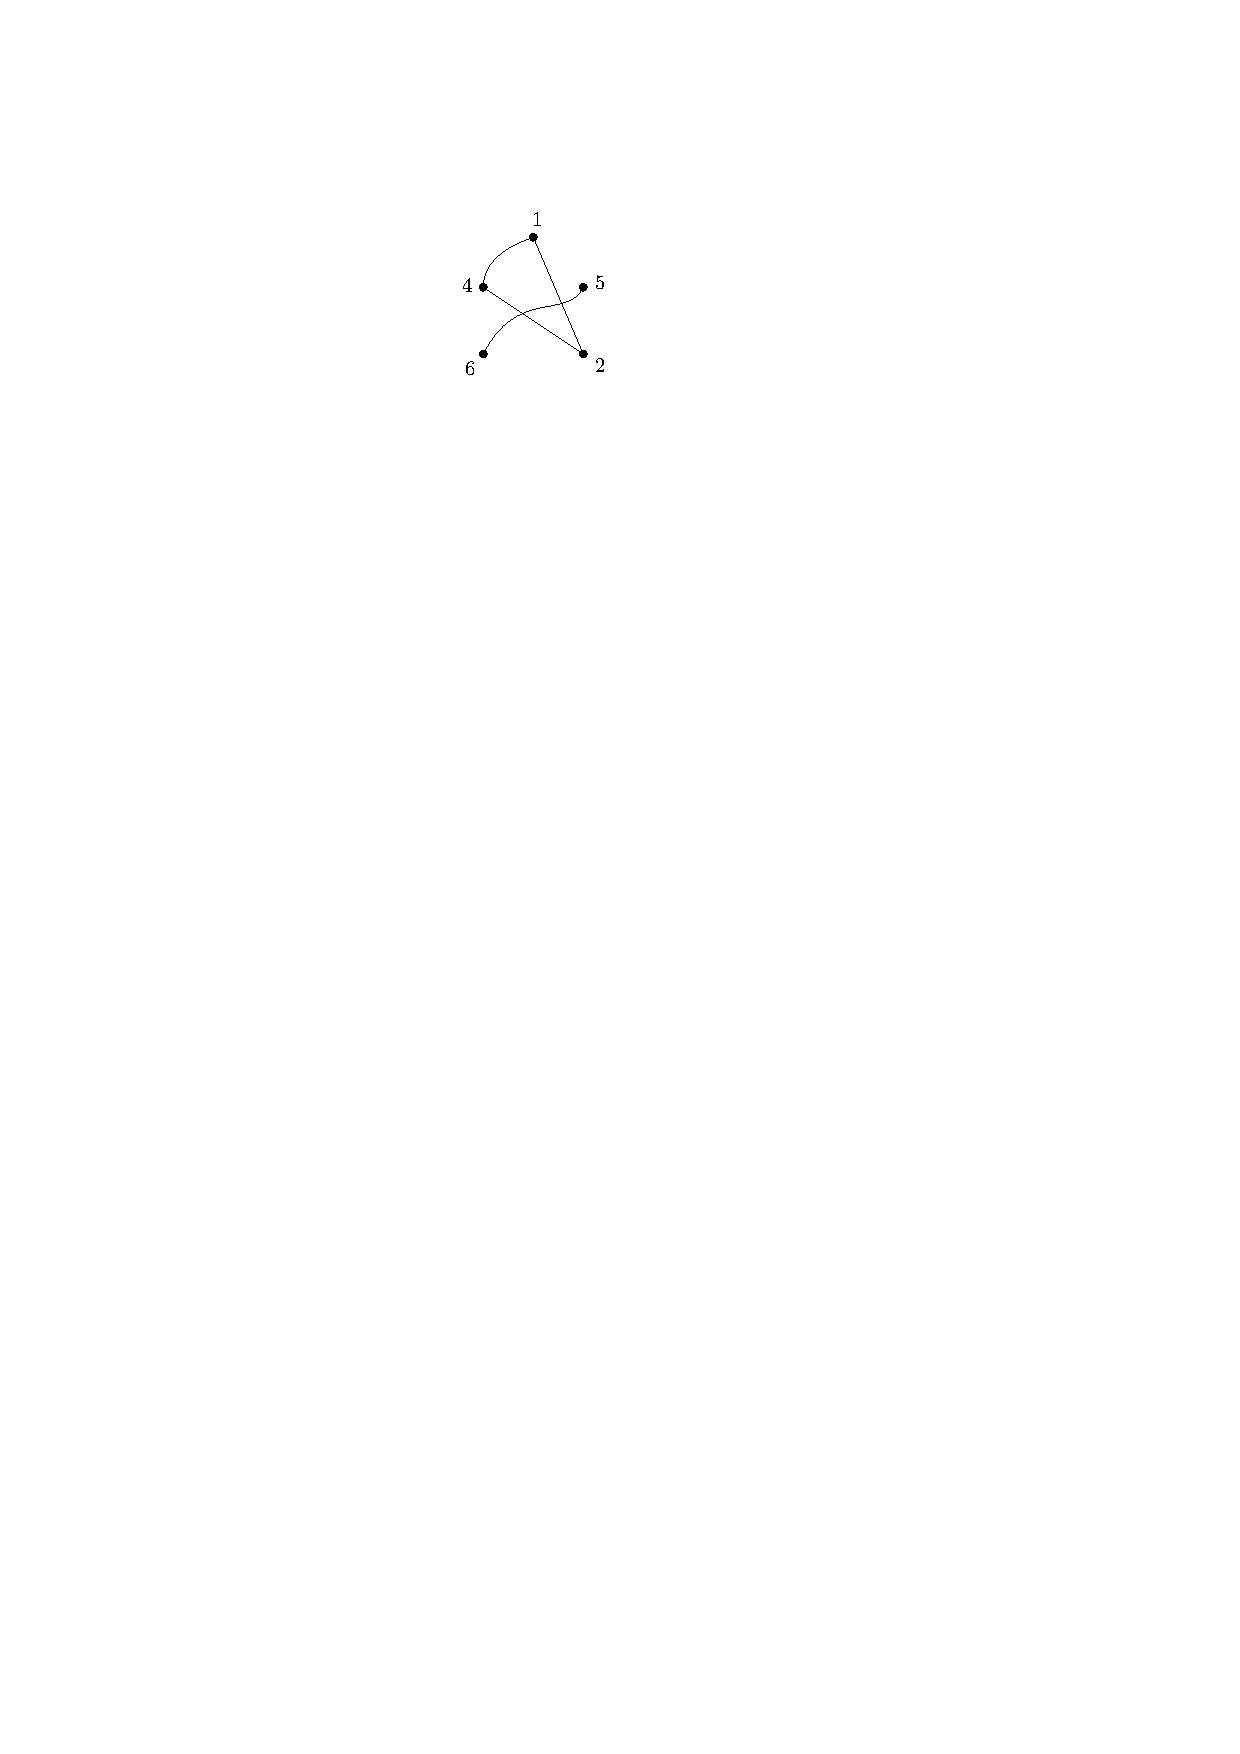
\includegraphics{umgrafo.pdf}
    \caption{um diagrama para o grafo do Exemplo~\ref{exem:umgrafo}.}
    \label{fig:umgrafo}
\end{figure}
\end{exem}

Para simplificar a notação, é comum escrever $uv$ (ou~$vu$) em vez de $\{u,v\}$ para denotar um par não ordenado.

Se $uv$ é uma aresta do grafo, diz-se que $u$ e $v$ são \emph{adjacentes} ou \emph{vizinhos} ou ainda que $u$ e $v$ estão ``ligados por uma aresta'' no grafo. Também se diz que $u$ e $v$ são \emph{extremidades} da aresta $uv$ e que $u$ e $v$ \emph{incidem} na aresta $uv$.  A \emph{vizinhança} de um vértice $u \in V$ é o conjunto de vizinhos de $u$, que é denotado por $N(u)$:
\[ N(u) = \{v \in V \colon uv \in E\}. \]
Quando a vizinhança de $u$ é o conjunto vazio, dizemos que $u$ é um \emph{vértice isolado}. Quando a vizinhança de~$u$ é ``todo mundo'' -- ou seja, quando $N(u) = V \setminus \{u\}$ -- dizemos que $u$ é um \emph{vértice universal}.

Neste curso, vamos tratar somente de grafos com conjunto de vértices finitos, mas é bom saber que grafos podem ser finitos ou infinitos. Em se tratando de grafos finitos, é comum denotar o número de vétrtices por $n$ (também chamado de \emph{ordem} do grafo) e o número de arestas por $m$ (também chamado de \emph{tamanho} do grafo). 

%% B&M 1.1.1
\begin{exer}
Mostre que $m \leq \binom{n}{2}$.
\end{exer}

\subsection{Exemplos}

%$\rhd$ Grafo vazio $E_n$ 
\begin{figure}[H]
    \centering
    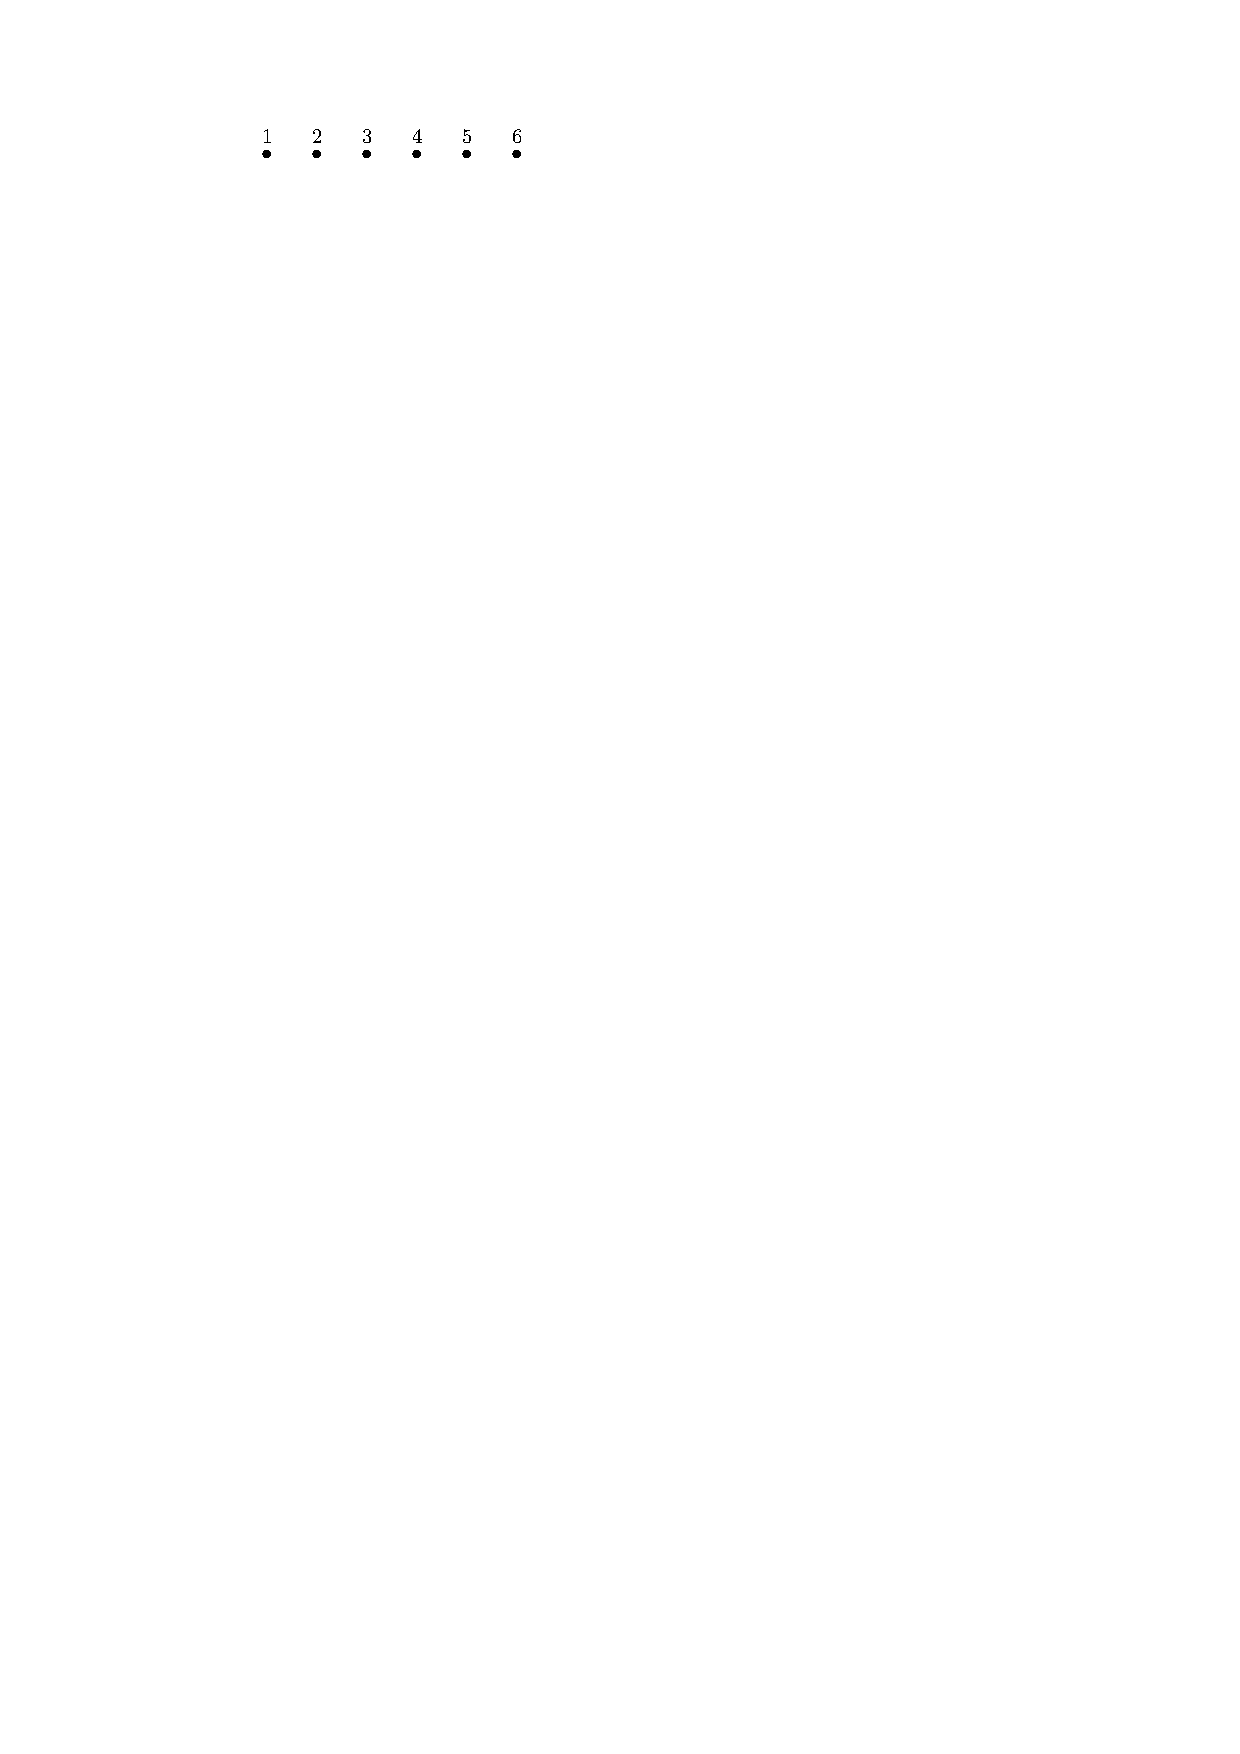
\includegraphics{vazio.pdf}
    \caption{o grafo vazio de ordem~$6$, chamado~$E_6$.}
    \label{fig:vazio}
\end{figure}
%\noindent $\rhd$ Grafo completo $K_n$ 
\begin{figure}[H]
    \centering
    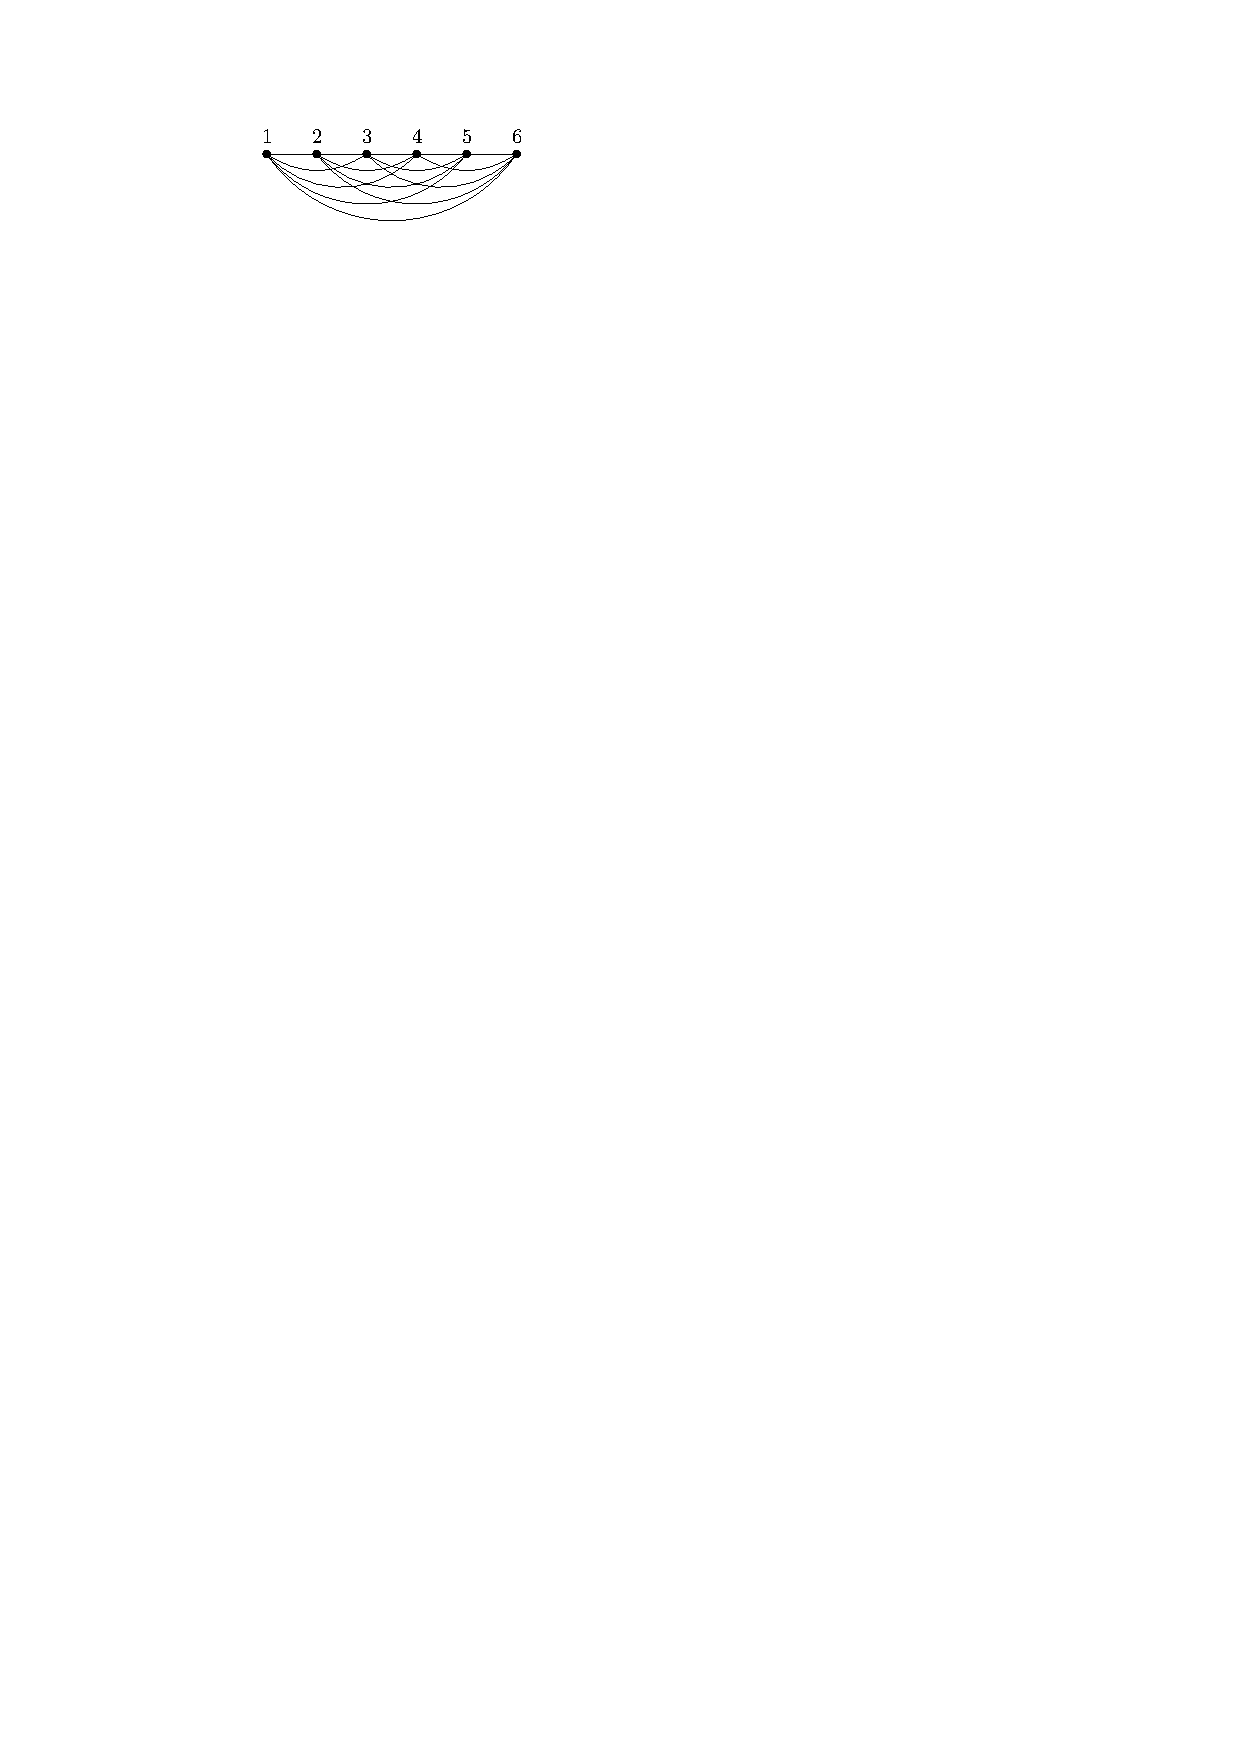
\includegraphics{completo.pdf}
    \caption{o grafo completo de ordem~$6$, chamado~$K_6$.}
    \label{fig:completo}
\end{figure}
%\noindent $\rhd$ O caminho $P_n$ 
\begin{figure}[H]
    \centering
    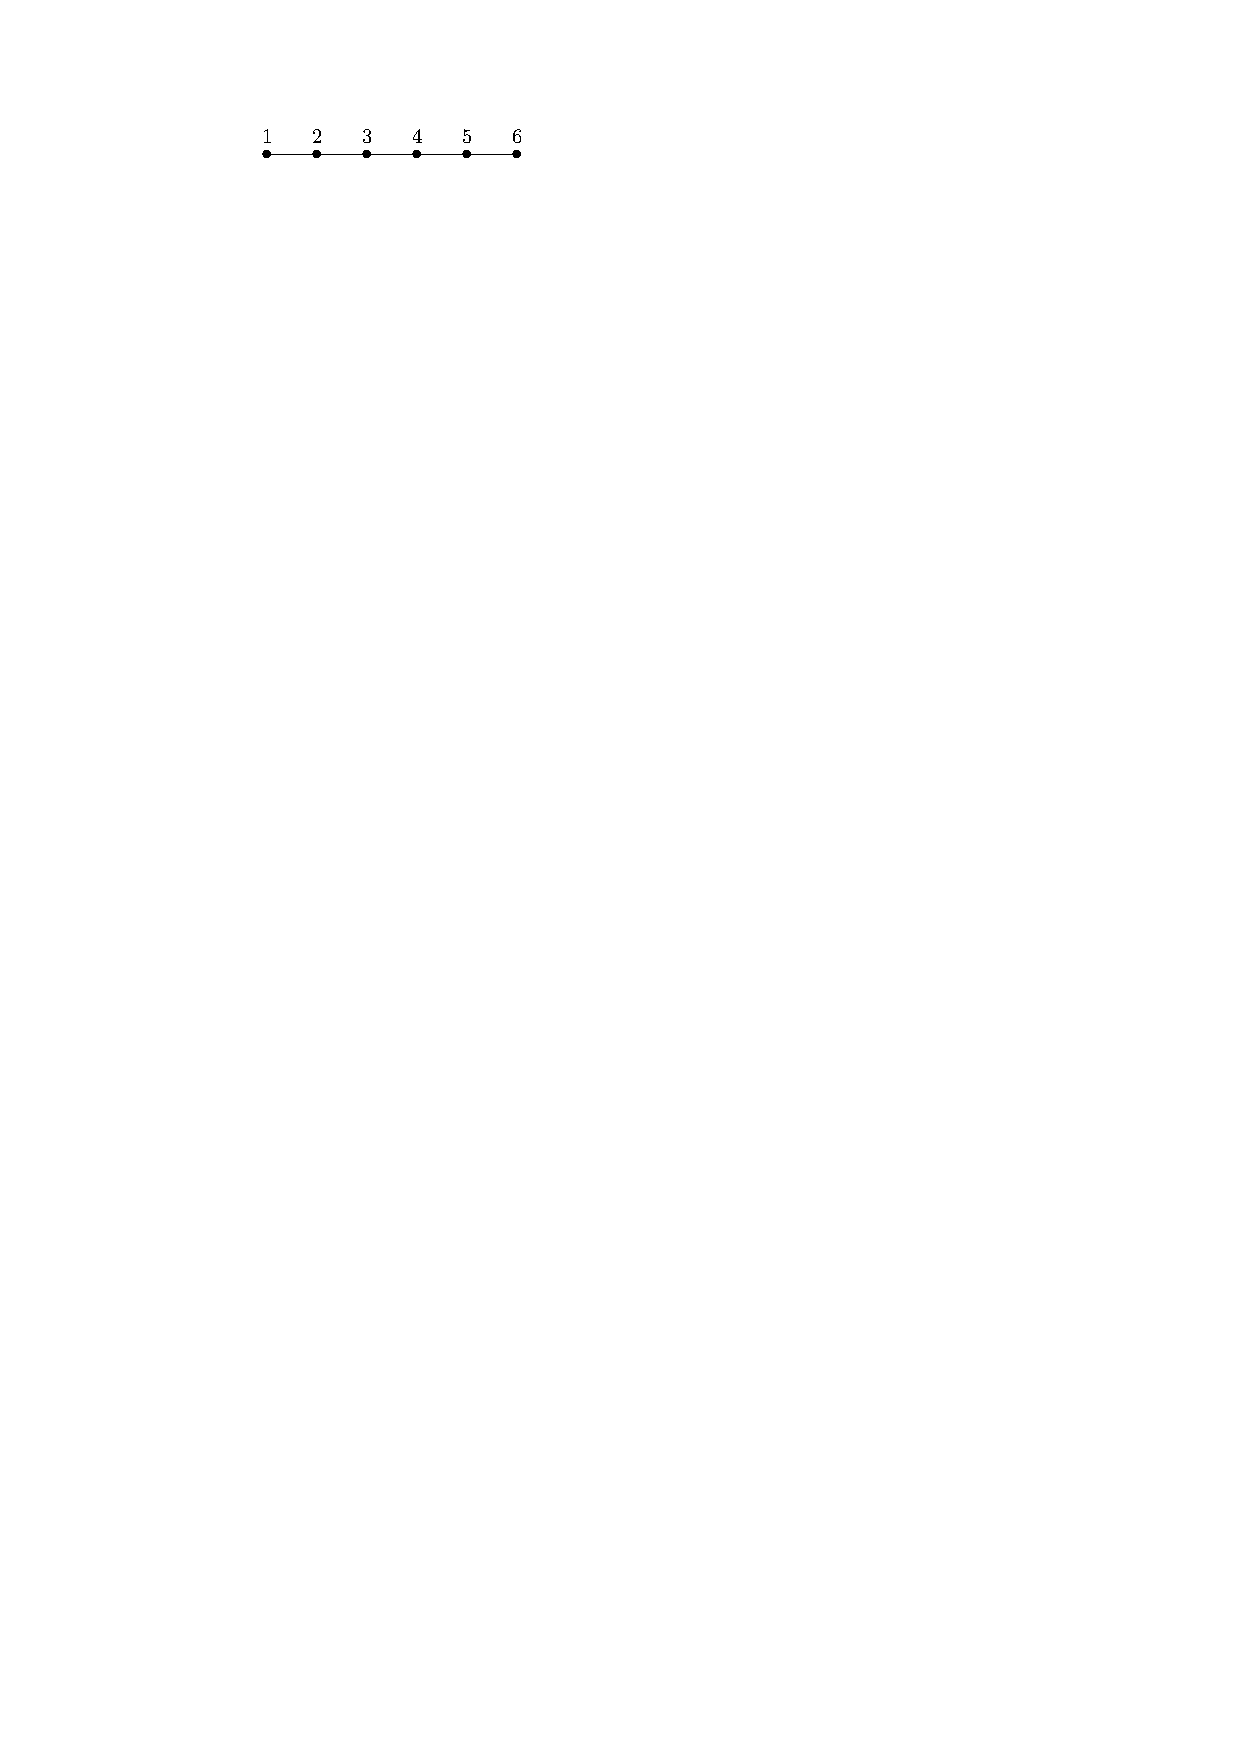
\includegraphics{caminho.pdf}
    \caption{o grafo caminho de ordem~$6$, chamado~$P_6$.}
    \label{fig:caminho}
\end{figure}
%\noindent $\rhd$ O circuito $C_n$
\begin{figure}[H]
    \centering
    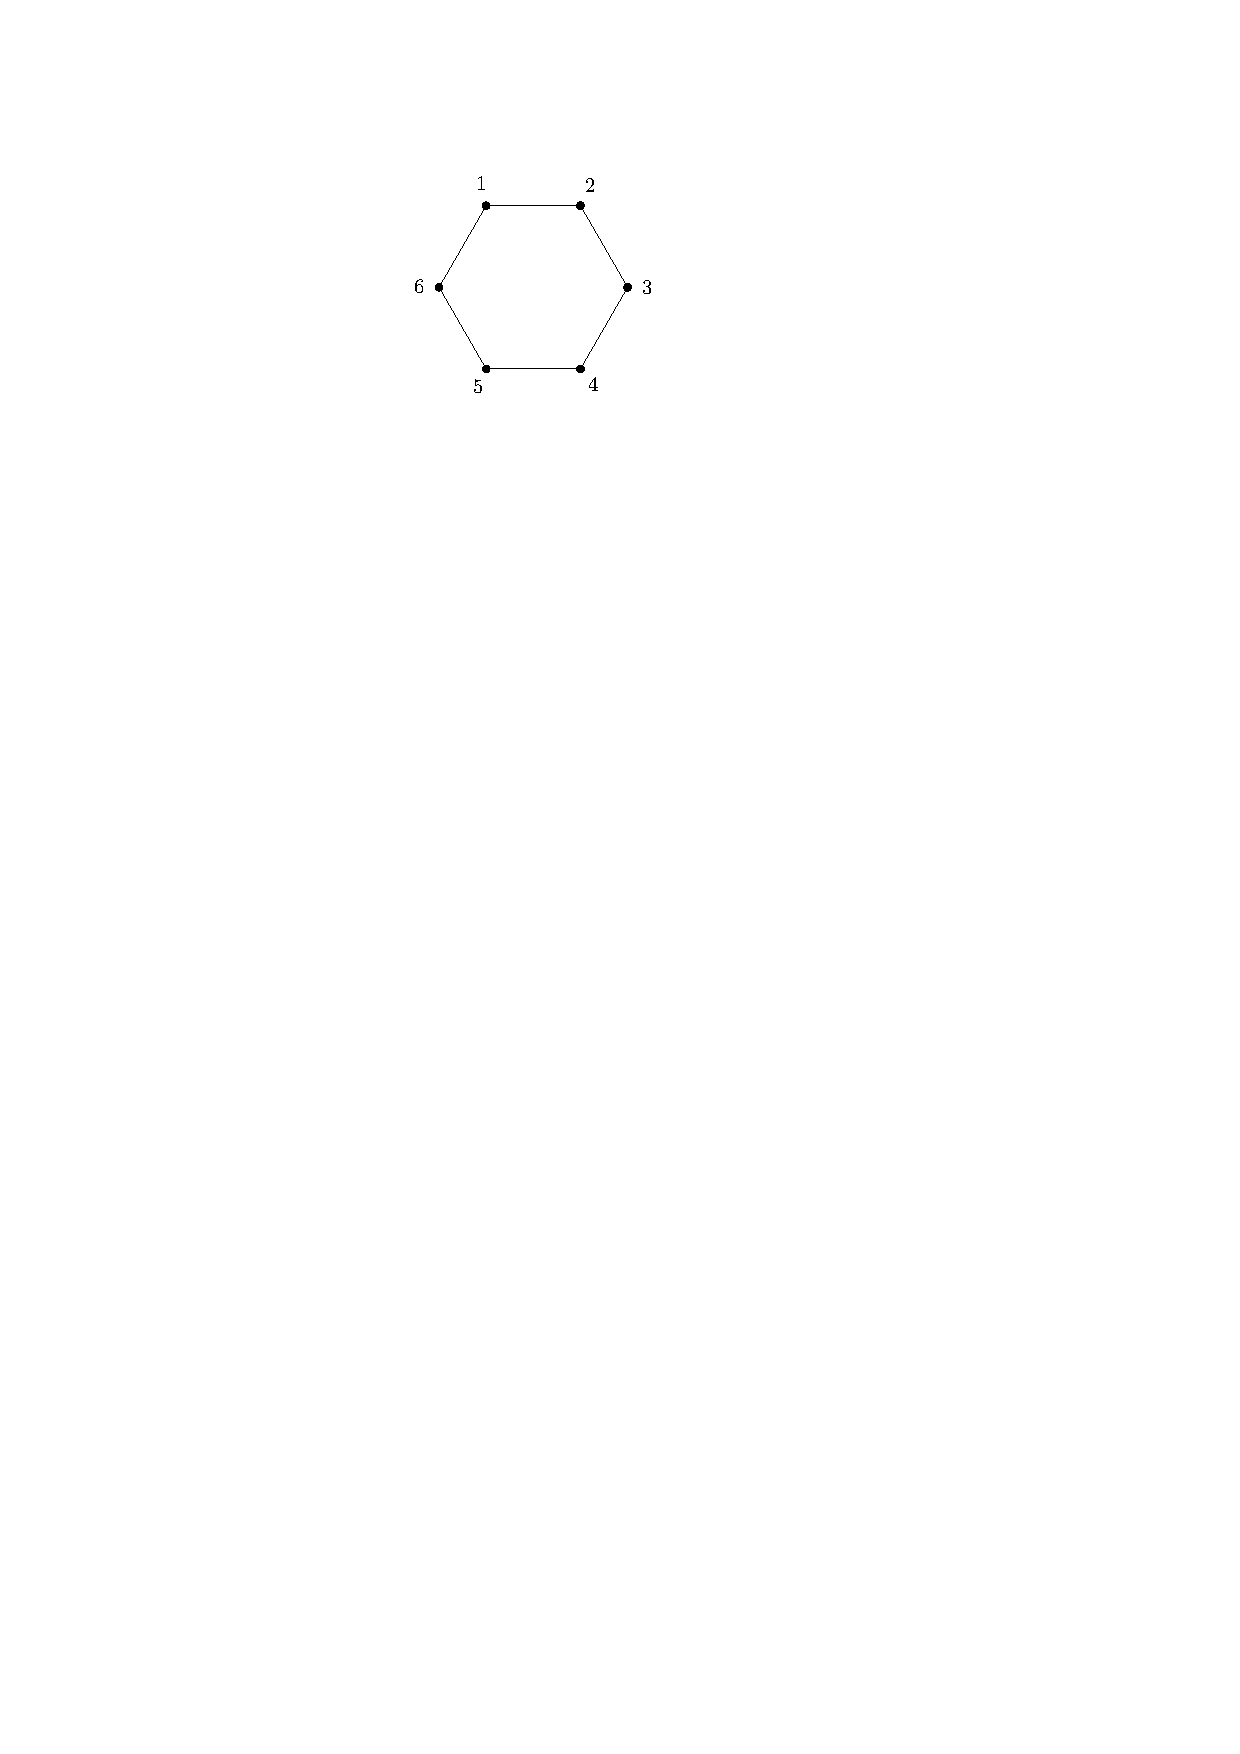
\includegraphics{circuito.pdf}
    \caption{o grafo circuito de ordem~$6$, chamado~$C_6$.}
    \label{fig:circuito}
\end{figure}
%\noindent $\rhd$ A estrela $S_{n-1}$ 
\begin{figure}[H]
    \centering
    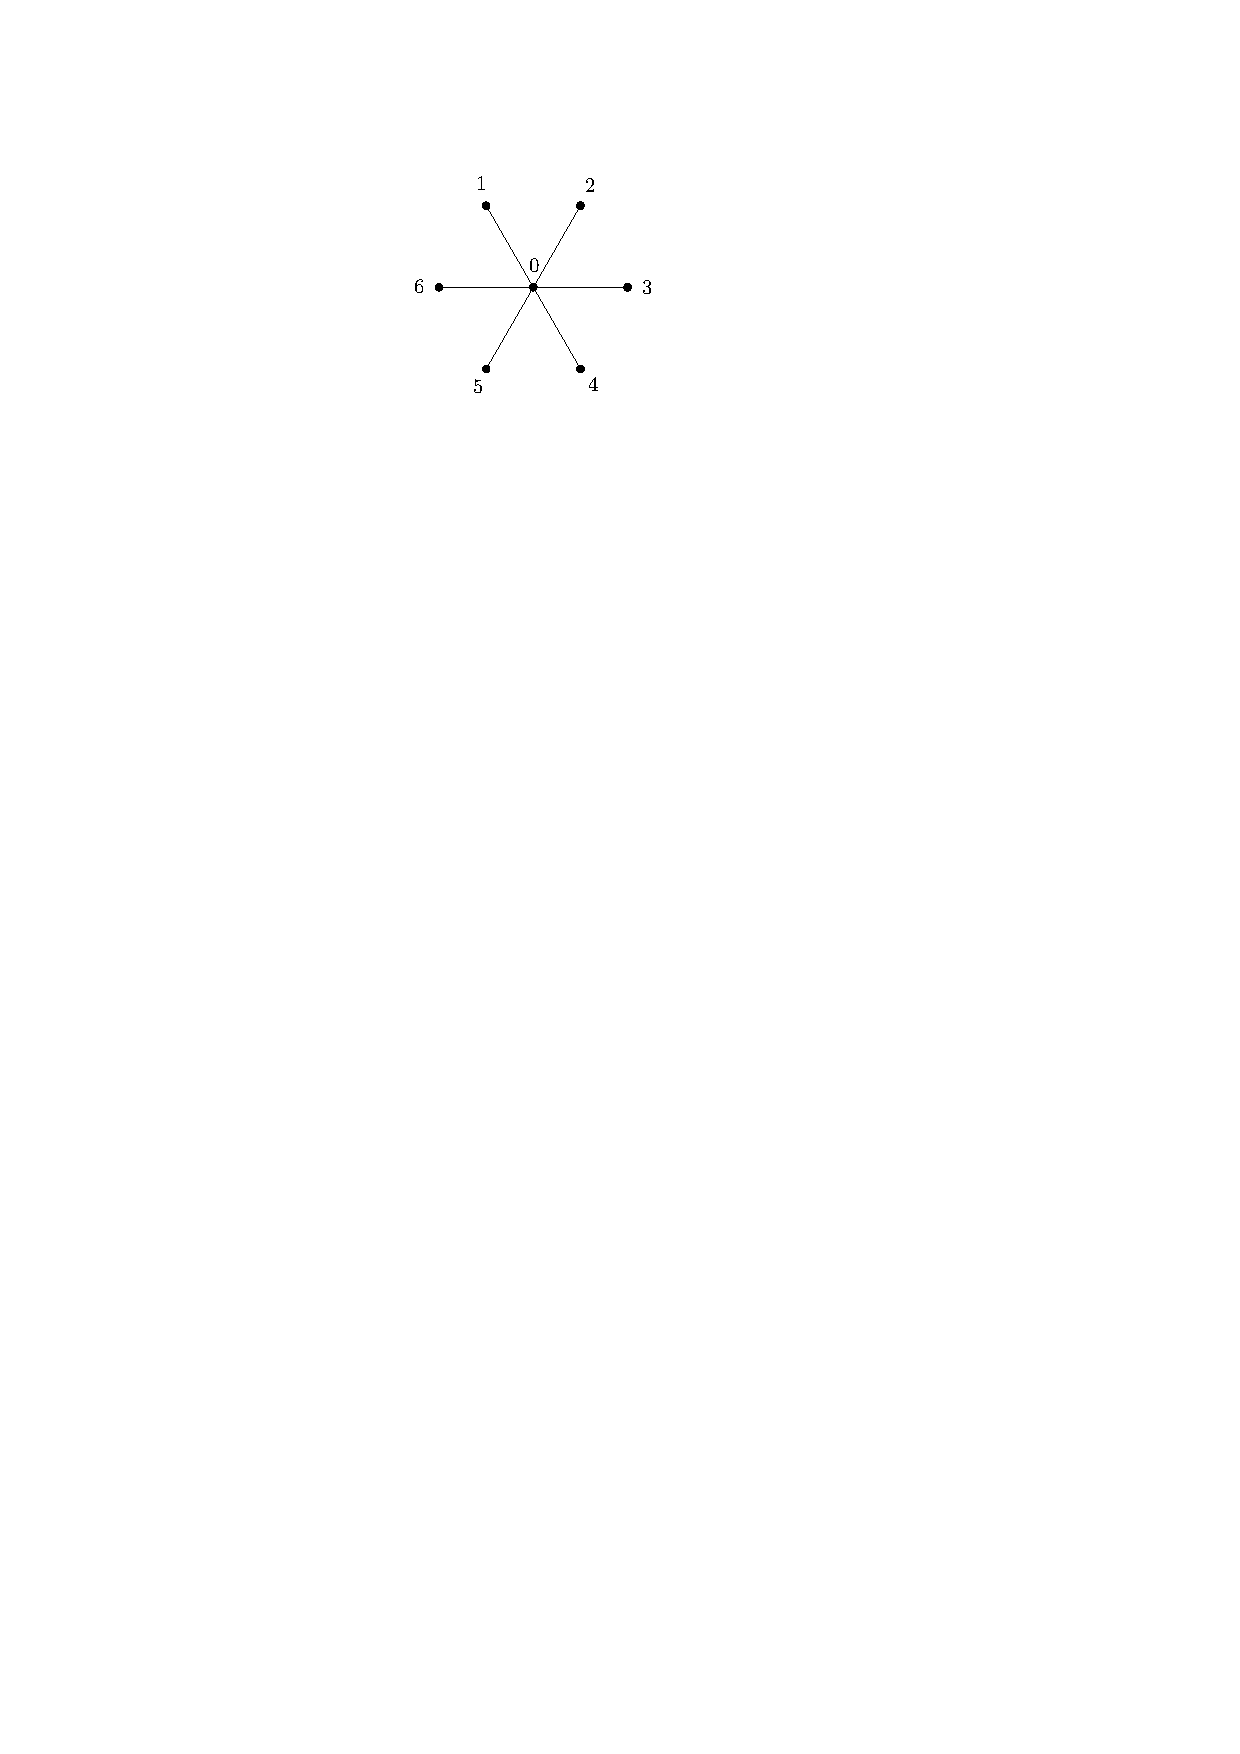
\includegraphics{estrela.pdf}
    \caption{o grafo estrela de ordem~$7$, chamado~$S_6$.}
    \label{fig:estrela}
\end{figure}

\begin{figure}[H]
    \centering
    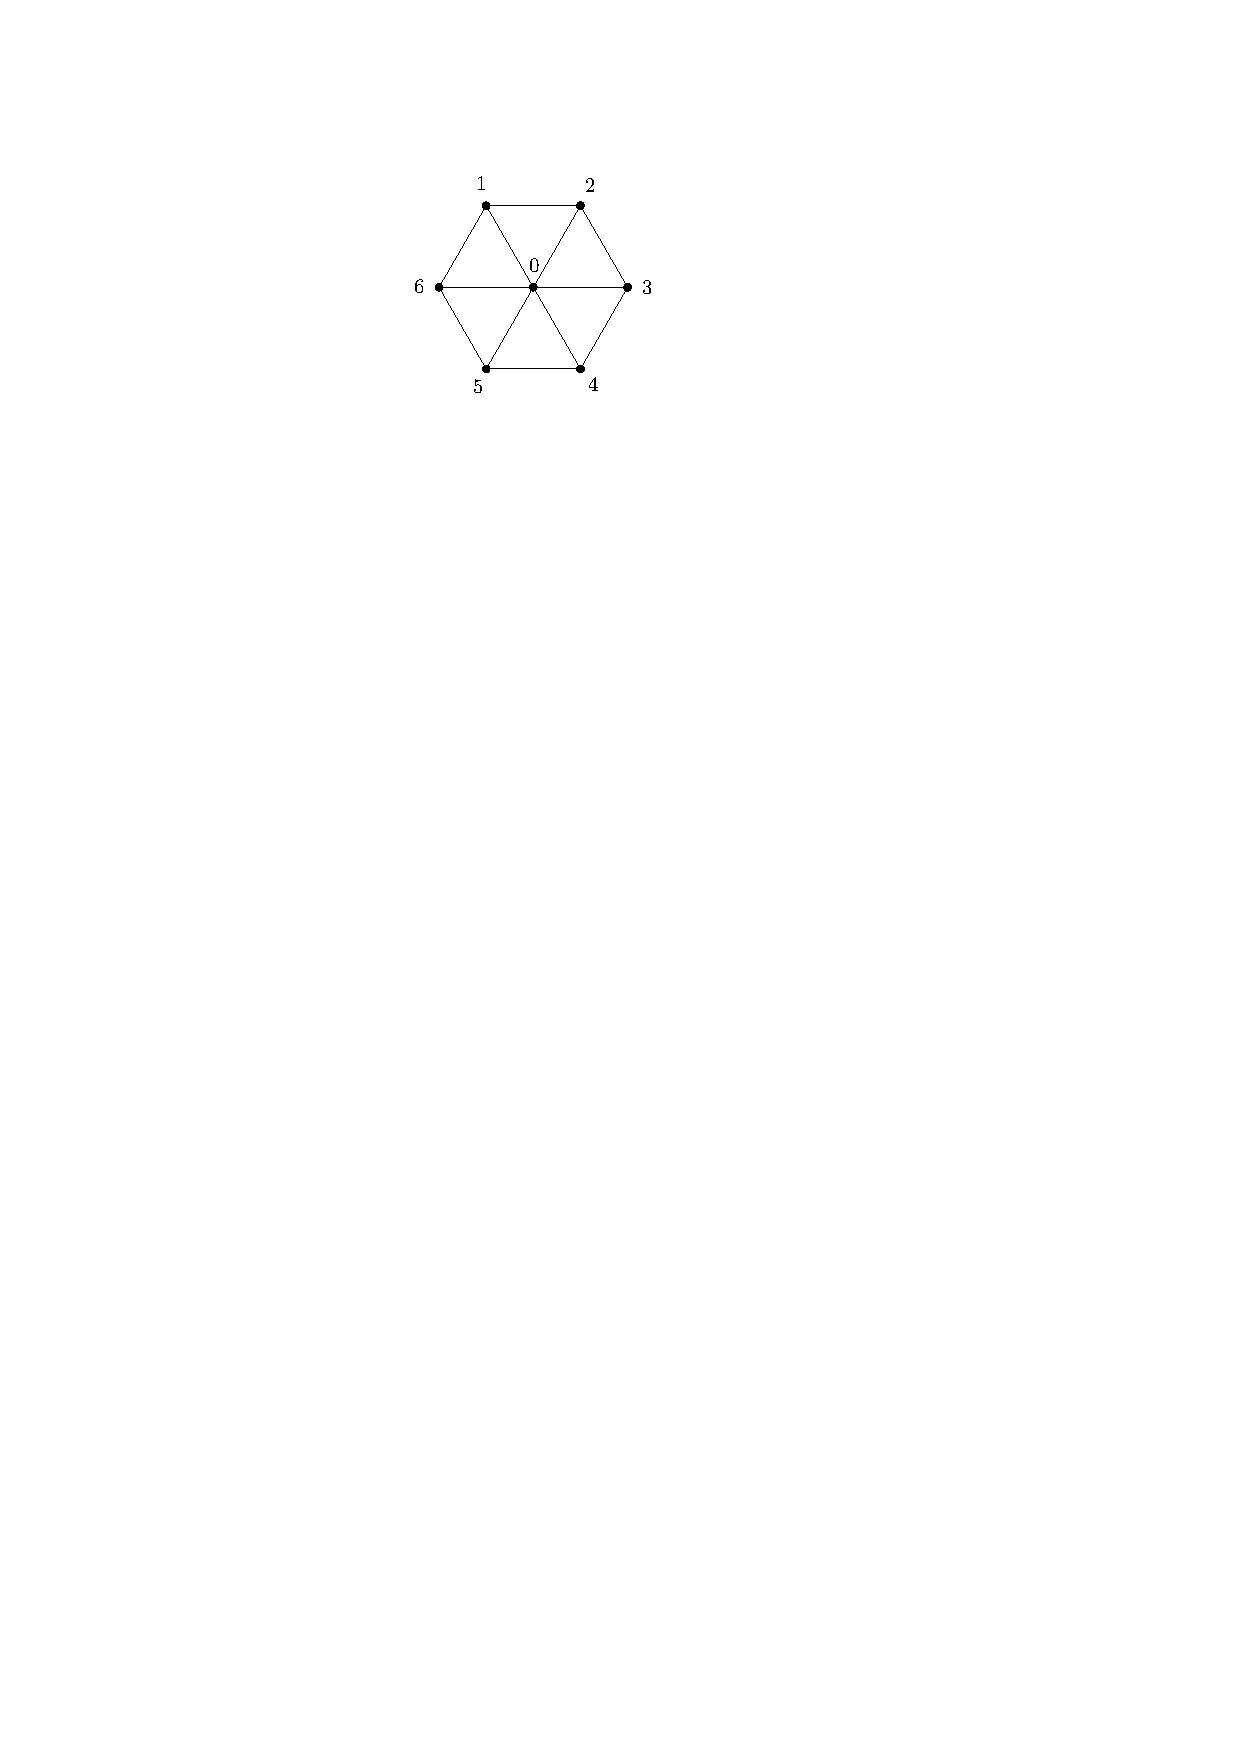
\includegraphics{roda.pdf}
    \caption{o grafo roda de ordem~$7$, chamado~$W_7$.}
    \label{fig:roda}
\end{figure}
%\noindent $\rhd$ A grade $G_{s \times t}$
\begin{figure}[H]
    \centering
    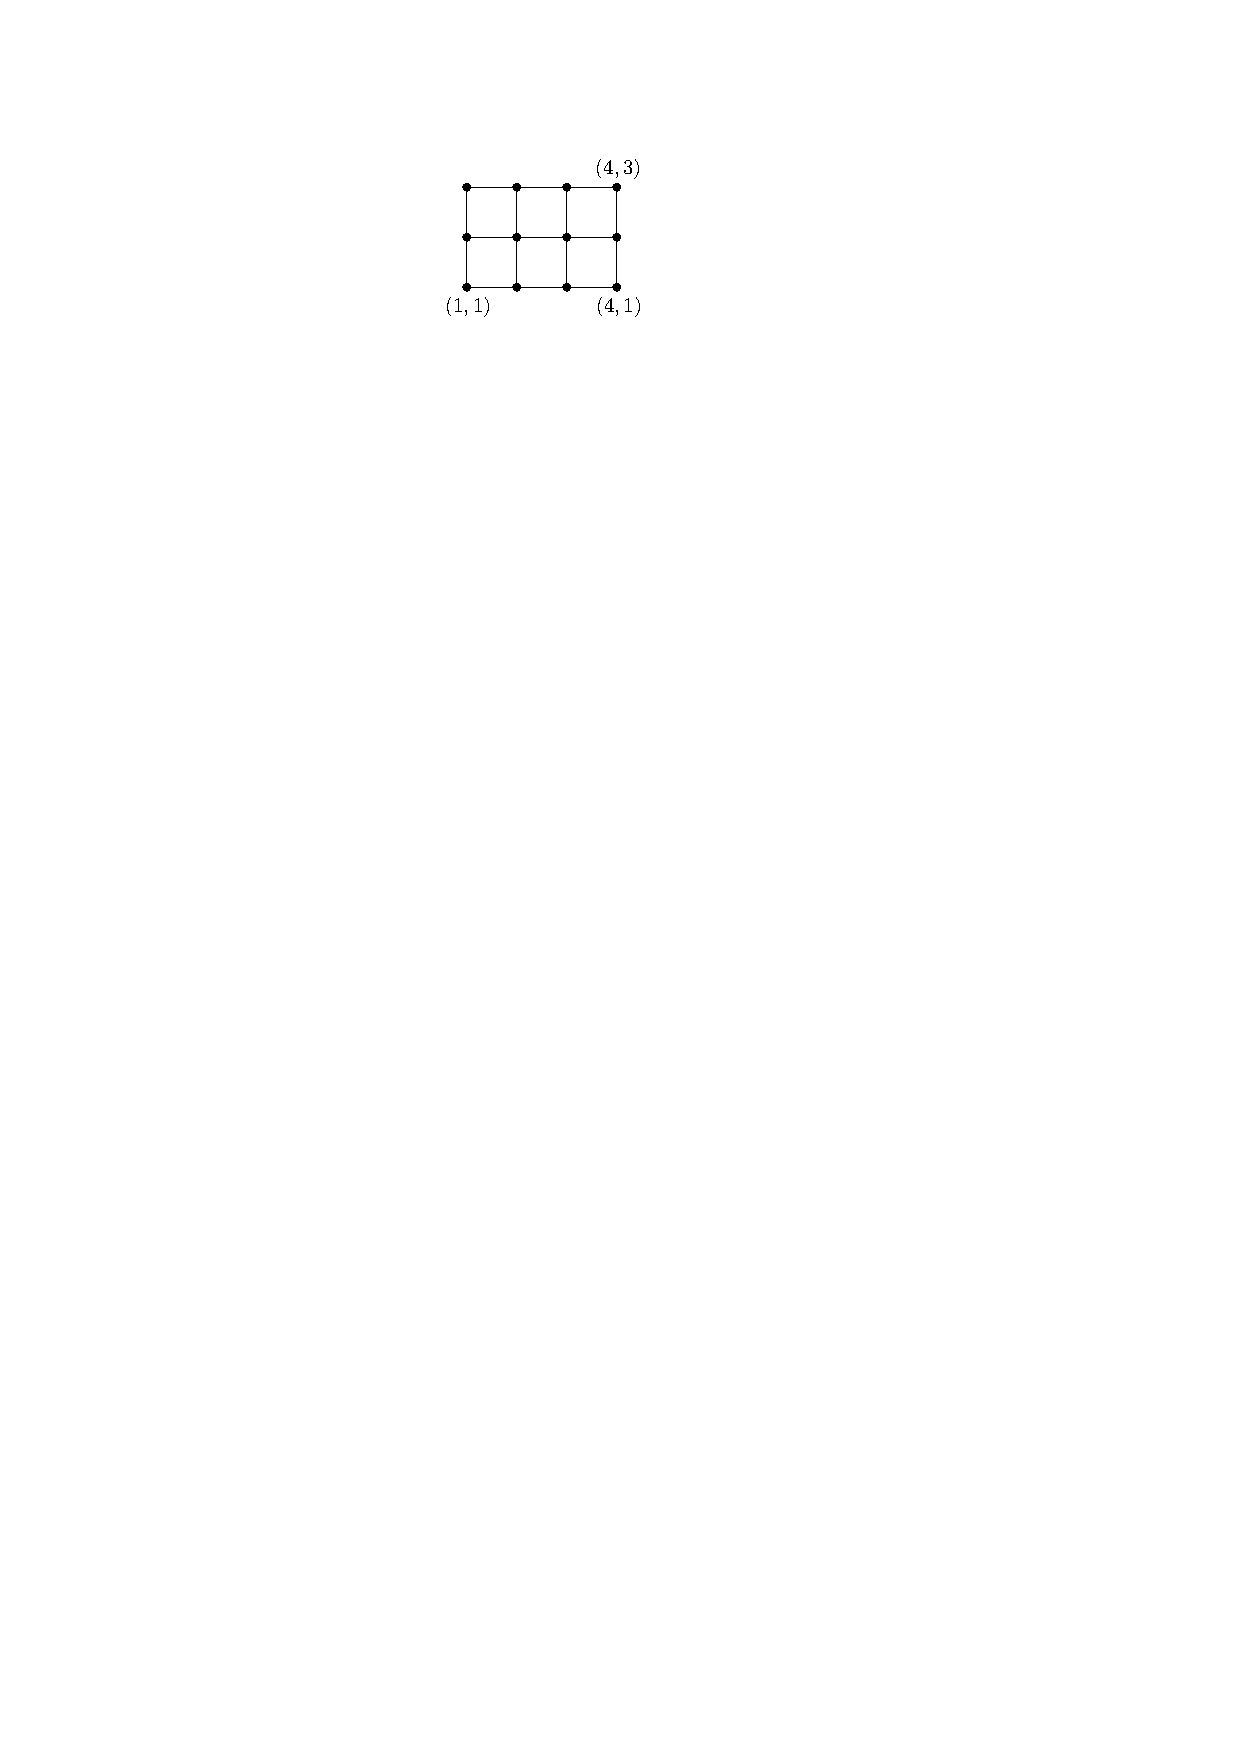
\includegraphics{grade.pdf}
    \caption{o grafo grade $3\times 4$, chamado~$G_{3\times 4}$.}
    \label{fig:grade}
\end{figure}
\subsection{Grau}

O número de arestas incidentes num vértice $v$ é chamado de \emph{grau} de $v$ e é denotado por $d(v)$. De acordo com a definição de grafo, esse número coincide com o número de vizinhos de $v$. O maior grau de um vértice num grafo é denotado por $\Delta$ e o menor grau, por $\delta$.

\begin{exem}
O grau de um vértice isolado é $0$, enquanto que o grau de um vértice universal é $n - 1$. Se um grafo tem um vértice isolado, como o grafo vazio, então $\delta = 0$. 
\end{exem}

\begin{exer}
Para cada grafo na seção anterior, diga quanto valem $\delta$ e $\Delta$.
\end{exer}

%% B&M 1.1.6 (a)
\begin{exer}
Mostre que, para qualquer grupo com duas ou mais pessoas, há sempre um par delas com o mesmo número de amigos no grupo.
\end{exer}

\begin{prop}
\label{prop:parity_sum_degrees}
A soma dos graus dos vértices de um grafo $(V,E)$ é par.
\end{prop}

\begin{proof}
Considere uma matriz $M$ com dimensões $n \times m$, em que cada linha corresponde a um vértice de $V$ e cada coluna corresponde a uma aresta de $E$. Para cada vértice $v \in V$ e aresta $e \in E$, a entrada $M_{ve}$ vale $1$ se $v$ incide em $e$ e vale $0$ caso contrário. Essa matriz é chamada de \emph{matriz de incidência} do grafo. 

Note que a linha da matriz correspondente ao vértice $v$ possui exatamente $d(v)$ entradas valendo $1$. Portando soma dos graus dos vértices do grafo nada mais é do que a quantidade de entradas iguais a $1$ nessa matriz. 

Por outro lado, cada coluna dessa matriz possui exatamente duas entradas valendo $1$, pois cada aresta $e$ incide em exatamente dois vértices. Assim, a quantidade de entradas que valem $1$ nessa matriz é $2m$, que é par. Segue que o enunciado da proposição é verdadeiro.
\end{proof}

\noindent Na verdade, a prova da proposição anterior nos dá mais informações do que simplesmente a paridade da soma dos graus em um grafo: ela nos dá que a seguinte igualdade é verdadeira para qualquer grafo.

\begin{equation}
    \label{eq:sum_degrees}
    \sum_{v \in V} d(v) = 2m. 
\end{equation} 

\begin{exer}
Mostre que, em qualquer grafo, é par a quantidade de vértices que possuem graus ímpares.
\end{exer}

\noindent Além do grau mínimo e máximo de um grafo, outro parâmetro bastante utilizado é o grau médio que, em vista da equação~\eqref{eq:sum_degrees}, pode ser calculado pela expressão $2m/n$.

%% B&M 1.1.4
\begin{exer}
Mostre que, para qualquer grafo, vale $\delta \leq 2m/n \leq \Delta$.
\end{exer}

\noindent Quando um grafo possui todos os seus vértices com o mesmo grau, dizemos que esse grafo é \emph{regular}. No caso do grau de todo vértice ser um inteiro~$k$, podemos dizer que o grafo é $k$-regular.

%% B&M 1.1.5
\begin{exer}
Para $k = 0,1,2$, caracterize os grafos $k$-regulares.
\end{exer}

\begin{exer}
Quantas arestas possui um grafo $k$-regular de ordem $n$?
\end{exer}

\section {Notação }

Nas seções anteriores, bastante notação foi definida para que possamos nos referir às diversas partes, invariantes e coisas relativas a um grafo. No entanto, frequentemente, no contexto dos problemas e resultados que vamos investigar neste curso, surge a necessidade de fazer referência a mais de um grafo simultaneamente e, quando escrevemos $\Delta$, $d(v)$, $V$ ou $m$ precisamos saber exatamente a qual dos grafos envolvidos estamos nos referindo. Nesse caso, podemos usar subscrito em cada uma das notações definidas acima para especificar o grafo. Por exemplo, se precisamos usar dois grafos $G$ e $H$ numa mesma prova, podemos escrever $d_G(v)$ para falar do grau de $v$ no grafo $G$, ou $m_H$ para fazer referência ao número de arestas de $H$. O conjunto de vértices de $G$, deve ser denotado por $V_G$, o grau máximo de $H$, por $\Delta_H$, etc.


\section{Operações básicas}

A partir de grafos conhecidos, podemos realizar algumas operações para obter novos grafos. Uma operação bastante utilizada é a remoção de elementos do grafo, sejam eles vértices ou arestas. Dado um grafo $G$ e dado uma aresta $e \in E_G$, denotamos por $G - e$ o grafo $(V_G, E_G \setminus \{e\})$.

A remoção de um vértice $v$ é uma operação ligeiramente mais complicada, pois é necessário remover as arestas que incidem em $v$ a fim de evitar inconsistências. Portanto $G - v$ é o grafo $(V_G \setminus \{v\}, E')$, onde
\[ E' = \{ uw \in E_G \colon u \neq v, w \neq v \}. \]
Outra operação simples é a complementação. O \emph{complemento} de um grafo $G = (V,E)$ é o grafo $\overline{G} = (V, \overline{E})$, onde 
\[ \overline{E} = \big\{ uv \subseteq V \colon uv \not\in E\big\}. \]
Note que, de acordo com essa definição, o complemento de $\overline{G}$ é o próprio grafo $G$.

\begin{exer}
Mostre que o complemento de um grafo regular é regular.
\end{exer}

\begin{exer}
Calcule $m_{\overline{G}}, \Delta_{\overline{G}}$ e $\delta_{\overline{G}}$ em função de $m_G, \Delta_G$ e $\delta_G$.
\end{exer}

\section{Isomorfismo}

A palavra \emph{isomorfo} vem do grego: \emph{iso} significa ``igual'' ou ``mesmo'', e \emph{morfo} significa ``forma''. Portanto, ao dizermos que dois grafos são isomorfos, estamos transmitindo a idéia de que eles têm a mesma forma. Por exemplo, considere os grafos ilustrados na Figura~\ref{fig:dois_grafos} abaixo. Apesar dos diagramas serem diferentes e apesar dos nomes dos vértices não serem os mesmos, esses grafos possuem a mesma forma, a mesma estrutura subjacente.
\begin{figure}[H]
    \centering
    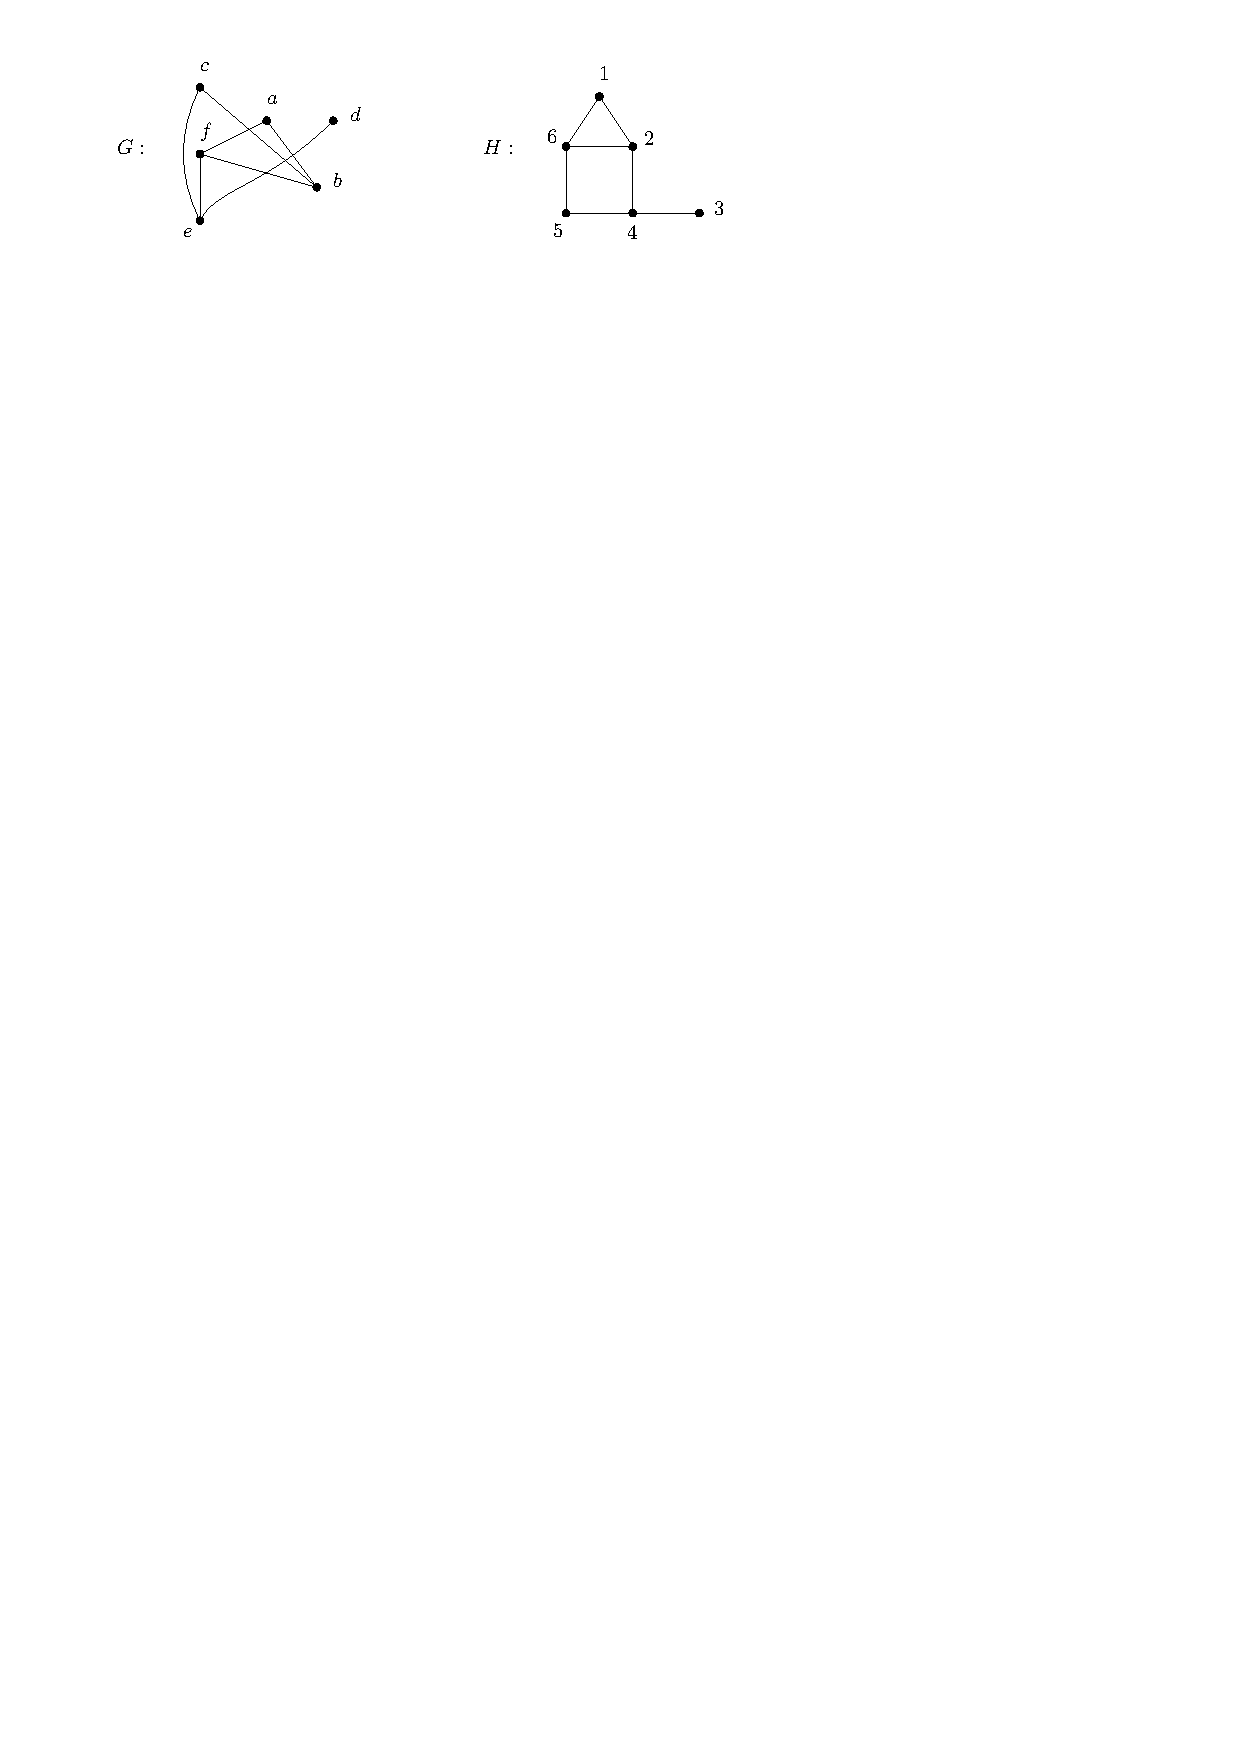
\includegraphics{isomorfos.pdf}
    \caption{dois grafos isomorfos.}
    \label{fig:dois_grafos}
\end{figure}

\noindent Dizemos que grafos $G$ e $H$ são \emph{isomorfos} se existe uma bijeção $\phi \colon V_G \rightarrow V_H$ tal que, para todo par de vértices $u, v \in V_G$, vale que
\begin{equation}
\label{eq:iso}
    uv \in E_G \iff \phi(u)\phi(v) \in E_H.
\end{equation} 
Uma função $\phi$ com essa propriedade é chamada de um \emph{isomorfismo} entre $G$ e $H$ e, quando ela existe, escrevemos $G \cong H$. Dizemos que uma bijeção satisfazendo~\eqref{eq:iso} \emph{respeita}
  ou \emph{preserva} a relação de adjacência.
\begin{exem}
Considere os grafo $G = (\{a, b, c, d\}, \{ab, ac, ad, bc\})$ e $H = (\{1, 2, 3, 4\}, \{12, 13, 14, 34\})$. Eles são grafos isomorfos pois podemos construir uma bijeção $\phi$ que satisfaz \eqref{eq:iso}, dada pela tabela a seguir.
\begin{table}[H]
    \centering
    \begin{tabular}{c||c|c|c|c}
        $x$ & $a$ & $b$ & $c$ & $d$ \\
        \hline
        $\phi(x)$ & $1$ & $3$ & $4$ & $2$
    \end{tabular}
    \caption{um isomorfismo entre $G$ e $H$.}
    \label{tab:phi1}
\end{table}
\end{exem}
\noindent Para verificar que a função $\phi$ dada pela tabela acima é, de fato, um isomorfismo, é necessário considerar cada possível par de vértices em $G$ e verificar se existe uma aresta ligando-os em $G$ se e só se os vértices correspondentes a eles em $H$ também estão ligados por uma aresta.

\begin{table}[H]
    \centering
    \begin{tabular}{c||c|c|c|c|c|c}
         $uv \subseteq V_G$ & $ab$ & $ac$ & $ad$ & $bc$ & $bd$ & $cd$ \\
         \hline
         $uv \in E_G$? & $\checkmark$ & $\checkmark$ & $\checkmark$ & $\checkmark$ &   &   \\
         \hline
         $\phi(u)\phi(v) \subseteq V_H$ & $13$ & $14$ & $12$ & $34$ & $32$ & $42$ \\
         \hline
         $\phi(u)\phi(v) \in E_H$? & $\checkmark$ & $\checkmark$ & $\checkmark$ & $\checkmark$ &   &   
    \end{tabular}
    \caption{verificação de que $\phi$ é isomorfismo.}
    \label{tab:verif}
\end{table}

\begin{exem}
$G_{2\times 2}$ e $C_4$ são isomorfos.
\end{exem}

\begin{exem}
Os grafos $C_5$ e $C_4$ não são isomorfos, pois possuem quantidades de vértices diferentes.
\end{exem}

\begin{exem}
Os grafos $C_5$ e $P_5$ não são isomorfos, pois possuem quantidades de arestas diferentes.
\end{exem}

\begin{exem}
Os grafos $S_5$ e $P_6$, apesar de terem exatamente o mesmo número de vértices e arestas, não são isomorfos, pois $S_5$ possui um vértice de grau $5$, mas $P_6$ não.
\end{exem}

\begin{exer}
Você conseguiria dar exemplos de grafos $G$ e $H$ com mesmo número de vértices e arestas, e com a mesma sequência de graus, mas que não são isomorfos?
\end{exer}

\begin{exer}
Mostre que os grafos da figura abaixo são isomorfos. (Basta exibir uma bijeção que é um isomorfismo, como fizemos na Tabela~\ref{tab:phi1}. Não é necessário verificar que sua bijeção é isomorfismo como fizemos na Tabela~\ref{tab:verif}.)
\begin{figure}[H]
    \centering
    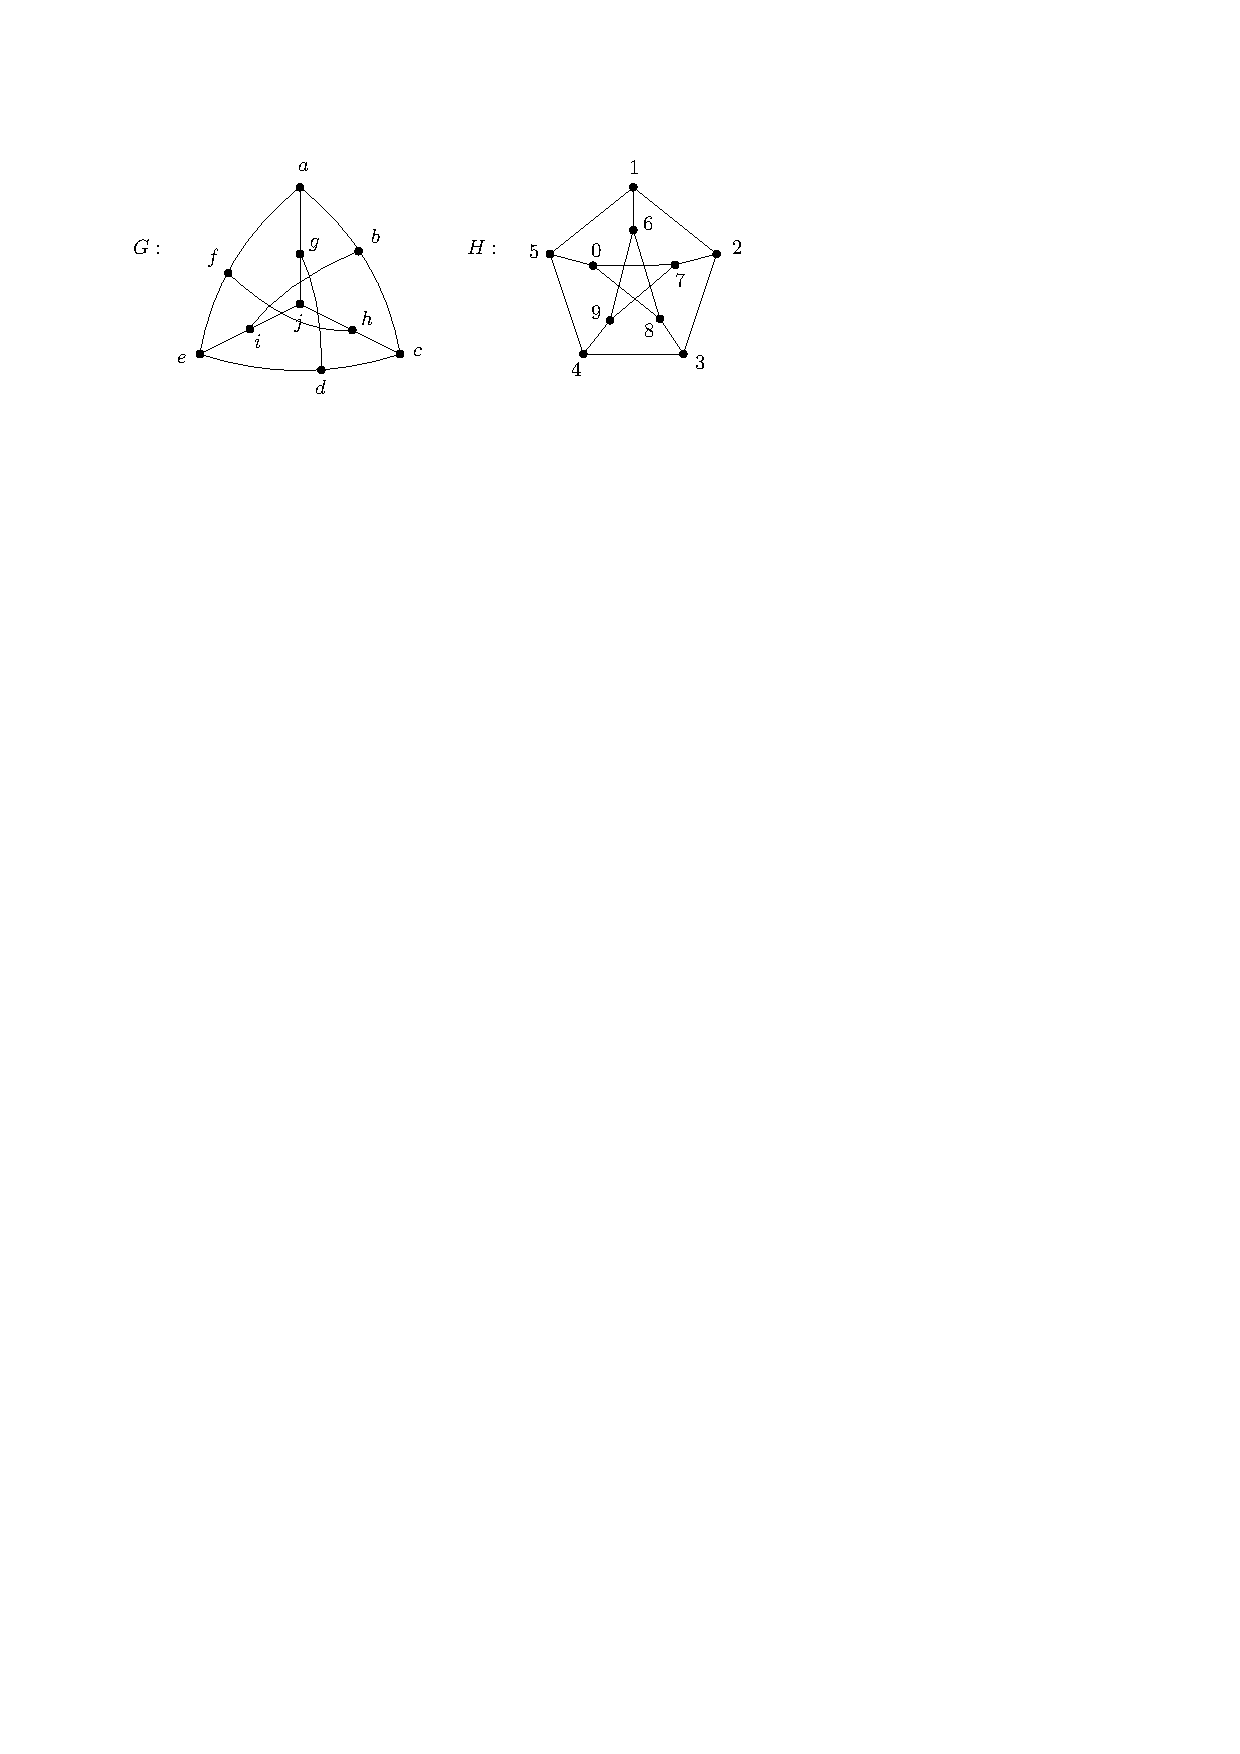
\includegraphics{petersen.pdf}
    \caption{dois grafos isomorfos.}
    \label{fig:pete}
\end{figure}
\end{exer}

\begin{exer}
  \label{exc:edge_map}
  Mostre que, se~$G$ é isomorfo a~$H$, então existe uma bijeção $\psi
  \colon E_G \rightarrow E_H$ satisfazendo
  \[
  \psi(e) \cap \psi(f) = \emptyset \iff e \cap f = \emptyset.
  \]
\end{exer}

\begin{exer}
  Mostre que a recíproca do Exercício~\ref{exc:edge_map} não é verdadeira.
\end{exer}

\noindent Muitas vezes dizemos que dois grafos são iguais, quando na verdade eles são apenas isomorfos. Isso se deve ao fato de que grafos isomorfos compartilham todas as suas propriedades (exceto, é claro, os nomes/rótulos de seus vértices).


\begin{exer}
  Mostre que~$C_n \not\cong C_m$ para~$n\neq m$. 
  % \emph{Resposta.}  Os grafos~$C_n$ e~$C_m$ não têm o
  % mesmo número de vértices, portanto não podem ser isomorfos.
\end{exer}

\begin{exer}
  Quantos grafos não-isomorfos existem com~$4$ vértices?
\end{exer}

\begin{exer}
  Exibir um grafo~$G$ de ordem~$4$ com~$G \cong \overline{G}$.
\end{exer}

\begin{exer}
  Exibir um grafo~$G$ de ordem~$5$ com~$G \cong \overline{G}$.
\end{exer}

\begin{exer}
  Prove que não existe~$G$ de ordem~$6$ com~$G \cong \overline{G}$.
\end{exer}

\section{Subgrafos}

Dizemos que $G$ é \emph{subgrafo} de $H$ se $V_G \subseteq V_H$ e $E_G \subseteq E_H$.

\begin{exem}
\label{exem:subgraph}
O grafo $F = (\{a, b, c, f\}, \{ab, bc\})$ é subgrafo do grafo $G$ da Figura~\ref{fig:pete}.
\end{exem}

\noindent Dado um grafo $G$ e dado um subconjunto de vértices $X \subseteq V_G$, chamamos de \emph{subgrafo induzido} por $X$ o subgrafo de $G$ que possui $X$ como conjunto de vértices e todas as possíveis arestas de $G$ que ligam pares de vértices em~$X$. Mais formalmente, o subgrafo de $G$ \emph{induzido} por $X$ é o grafo $G[X] = (X,E_G(X,X))$ onde $E_G(X,Y)$ denota o conjunto de arestas com uma extremidade em~$X$ e outra em~$Y$:
\[ E_G(X,Y) = \{ uv \in E_G \colon u \in X \text{ e } v \in Y\}. \]
Se $H = G[X]$ para algum $X \subseteq V_G$, podemos dizer que $H$ é \emph{subgrafo induzido} de $G$.

\begin{exer}
O grafo $F$ do Exemplo~\ref{exem:subgraph} não é subgrafo induzido do grafo~$G$ na Figura~\ref{fig:pete}. Você conseguiria dizer qual é o subgrafo induzido pelo conjunto  $X = \{a,b,c,f\}$ em $G$? 
\end{exer}

\begin{exer}
Para um grafo $G$ e vértice $v \in V_G$, escreva $G - v$ como um grafo induzido por um conjunto de vértices, ou seja, determine $X$ tal que $G - v = G[X]$.
\end{exer}

%\noindent De maneira análoga, dado um grafo $G$ e um subconjunto de arestas $F \subseteq E_G$, podemos definir o \emph{subgrafo gerado} por $F$ como sendo o grafo $G[F] = (V_G, F)$, ou seja, $G[F]$ é o subgrafo de $G$ que possui todos os vértices de $G$, mas possui somente as arestas do subconjunto $F$.

\subsection{A notação \texorpdfstring{$G \subseteq H$}{G subconjunto de H}}

A definição de subgrafos é análoga à definição de subconjuntos. Isso tanto é verdade que é quase tentador escrever $G \subseteq H$ para denotar que $G$ é subgrafo de $H$. De fato, podemos usar essa notação quando $G$ for subgrafo de $H$, mas essa notação denota algo mais geral.

Em Teoria de Grafos, é mais comum nos preocuparmos com a forma (\emph{morfo}) do grafo do que com os rótulos dos vértices. Por esse motivo, às vezes escrevemos que ``$G$ é subgrafo de $H$'' quando, na verdade, deveríamos escrever ``$G$ é isomorfo a um subgrafo de $H$''. Vamos usar a notação $G \subseteq H$ para significar justamente isso: que $G$ é isomorfo a um subgrafo de $H$. Também dizemos, nesse caso, que $H$ contém uma \emph{cópia} de $G$.

\section{Passeios, caminhos, circuitos e trilhas}

Um \emph{passeio} num grafo~$G$ é uma seqüência~$v_0 v_1
\cdots v_k$ de vértices em~$V_G$ com~$v_{i-1} v_i \in E_G$ para todo~$i \in \{1,2,\dots,k\}$. Portanto, o que torna uma sequência de vértices um passeio em~$G$ é a restrição de que vértices consecutivos da sequência devem estar ligados por uma aresta no grafo. Desse modo, dizemos que as arestas \emph{percorridas} por esse passeio são as arestas $v_0v_1, v_1v_2, \dots, v_{k-1}v_k$.  

Seja $P = v_0v_1 \cdots v_k$ um passeio em um grafo $G$. Os vértices $v_0$ e $v_k$ são chamados de \emph{extremidades} do passeio. Para vértices~$u,v \in V_G$, um $(u,v)$-\textit{passeio} em~$G$ é um passeio cujas extremidades são~$u$ e~$v$. Dizemos que $P$ é \emph{fechado} se $v_0 = v_k$, caso contrário, dizemos que ele é \emph{aberto}. Quando os vértices de $P$ são dois a dois distintos, dizemos que $P$ é um \emph{caminho}. Quando os vértices de $P$ são dois a dois distintos exceto por $v_0 = v_k$, dizemos que $P$ é um \emph{circuito} ou um \emph{ciclo}. Quando as arestas percorridas por $P$ são duas a duas distintas, dizemos que $P$ é uma \emph{trilha}. O \emph{comprimento} de $P$ é o número arestas percorridas por $P$ (contando-se repetições); portanto, o comprimento de $P$ acima é $k$. Denotamos o comprimento de $P$ por $|P|$.

\begin{exem}
\label{exem:walk}
A sequência $edgjhcdga$ é um $(e,a)$-passeio de comprimen\-to~$8$ no grafo~$G$ da Figura~\ref{fig:pete}.
\end{exem}

\begin{prop}
Seja $G$ um grafo e sejam $u,v \in V_G$ dois vértices distintos. O grafo $G$ possui um $(u,v)$-passeio se e somente se $G$ possui um $(u,v)$-caminho.
\end{prop}

\begin{proof}
Primeiramente, observe que, por definição, todo caminho é um passeio. Portanto, se $G$ tem um $(u,v)$-caminho, então ele também possui um $(u,v)$-passeio.

Resta provar a recíproca: todo grafo que possui um $(u,v)$-passeio também possui um $(u,v)$-caminho. Para mostrar essa direção, vamos mostrar que qualquer $(u,v)$-passeio de comprimento mínimo em $G$ é um caminho. Seja $P = v_0v_1 \cdots v_k$ um $(u,v)$-passeio de comprimento mínimo em $G$ (note que $v_0 = u$ e $v_k = v$). Se os vértices dessa sequência são dois a dois distintos então acabou: $P$ é um caminho. Suponha, então, com a finalidade de chegarmos a uma contradição, que algum vértice do grafo apareça repetidas vezes em $P$, ou seja, suponha que existam índices $i < j$, com $0 \leq i < j \leq k$, tais que $v_i = v_j$. 
Considere a sequência $P'$ definida por $P' = v_0 \cdots v_i v_{j+1} \cdots v_k$. Vamos argumentar que:
\begin{enumerate}[(i)]
    \item \label{af:pl_menor} $P'$ tem comprimento menor que $P$, e
    \item \label{af:pl_passeio} $P'$ é um $(u,v)$-passeio em $G$.
\end{enumerate}
A existência de $P'$ é suficiente para chegarmos a uma contradição, pois $P$ foi escolhido de forma a ser um $(u,v)$-passeio de comprimento mínimo, o que significa que não pode haver outro $(u,v)$-passeio com comprimento menor que~$P$.

Resta, então, mostrar a validade de~\eqref{af:pl_menor} e~\eqref{af:pl_passeio}. Não é difícil ver que $P'$ tem comprimento menor que $P$, pois o comprimento de $P'$ é $i + k - j$, o que é menor que $k$ pelo fato de que $i < j$. Portanto a afirmação~\eqref{af:pl_menor} é verdadeira. Para argumentar que~\eqref{af:pl_passeio} é verdadeira, observe que todas os pares de vértices consecutivos em $P'$ são também consecutivos em $P$, inclusive o par $v_i v_{j+1}$, pois $v_i v_{j+1} = v_j v_{j+1}$. Portanto, todos os pares de vértices consecutivos da sequência $P'$ são arestas de $G$, o que torna $P'$ um passeio.

A prova da proposição está concluída.
\end{proof}

\begin{exer}
Mostre que $G$ tem uma trilha fechada se e somente se $G$ possui um circuito.
\end{exer}



\section{Conexidade}
\label{conn}

Uma \emph{partição} de um conjunto $V$ é uma coleção de subconjuntos não vazios de $V$, dois a dois disjuntos, cuja união é o próprio $V$. Cada um desses subconjuntos de~$V$ é chamado de \emph{parte}. Por exemplo, $\big\{\{1, 5, 7\}, \{2, 6\}, \{3, 4, 8\}\big\}$ é uma partição do conjunto $\{1, 2, \dots, 8\}$ nas partes $\{1, 5, 7\}, \{2, 6\}$ e $\{3, 4, 8\}$.

Um grafo $G$ é \emph{conexo} se, para toda partição de $V_G$ em duas partes~$X$ e~$Y$, existe uma aresta $e \in E_G$ tal que $e \cap X \neq \emptyset$ e $e \cap Y \neq \emptyset$. Diz-se de uma tal aresta~$e$ que ela \emph{cruza} a partição $\{X,Y\}$, pois ela tem uma extremidade em $X$ e outra em $Y$.

Ou seja, um grafo é conexo se, para toda partição $\{X,Y\}$ de $V_G$, existe uma aresta que cruza $\{X,Y\}$. Se um grafo não é conexo, dizemos que ele é \emph{desconexo}.

\begin{exer}
Escreva formalmente o que significa um grafo~$G$ ser desconexo.
\end{exer}

\begin{exem}
O grafo $G$ com $V_G = \{a, b, c, d, e\}$ e $E_G = \{ab, be, ae, cd\}$ não é conexo pois, tomando $X = \{a, b, e\}$ e $Y = \{c, d\}$, podemos perceber que não existe nenhuma aresta com uma extremidade em $X$ e outra em $Y$. 
\end{exem}

\begin{exem}
  O grafo a seguir também é desconexo.
  \begin{figure}[H]
      \centering
      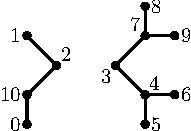
\includegraphics{desconexo-1.pdf}
      \caption{um grafo desconexo.}
      \label{fig:desc}
  \end{figure}
  \noindent Pra mostrar que esse grafo é desconexo devemos achar
  conjuntos~$X$ e~$Y$ tais que nenhuma aresta cruza~$\{X,Y\}$. Basta tomar~$X = \{0, 1, 2, 10\}$ e $Y = \{3, 4, 5, 6, 7, 8, 9\}$.
\end{exem}

\begin{exem}
O grafo da Figura~\ref{fig:pete}, mais conhecido como Grafo de Petersen, é um grafo conexo. 
\end{exem}

Como se convencer de que o Grafo de Petersen é conexo? Se quisermos usar diretamente a definição de grafo conexo, a única opção seria verificar que cada uma das partições do conjunto de vértices do Grafo de Petersen em dois conjuntos não vazios~$X$ e~$Y$ tem uma aresta que a cruza. 

\begin{exer}
Segundo a definição de grafo conexo, quantas partições deveriam ser analisadas para nos converncermos de que o Grafo de Petersen é conexo?
\end{exer}

A proposição a seguir estabelece que a propriedade de um grafo ser conexo é equivalente à propriedade de que entre quaisquer dois vértices do grafo existe um caminho. Essa propriedade é mais fácil de ser testada computacionalmente.

\begin{prop}
  \label{conex_prop}
  Um grafo~$G$ é conexo se e somente se para todo par de vértices~$x,y \in V_G$ existe um $(x,y)$-passeio em~$G$.
\end{prop}

\begin{proof}
Vamos primeiro supor que~$G$ é conexo e vamos mostrar que para todo par de vértices~$x,y \in V_G$ existe um $(x,y)$-passeio em~$G$. Sejam~$x$ e~$y$ vértices quaisquer em~$G$. Podemos supor que $x$ e~$y$ são vértices distintos. Seja~$X$ o conjunto de todos os vértices que podem ser atingidos a partir de~$x$ por um passeio. E chame de~$\overline{X}$ o complemento de~$X$. 
\begin{align*}
  X &= \{z \in V_G \colon \text{~existe um~} (x,z)\text{-passeio em~} G \},\\
    \overline{X} &= V_G \setminus X.
  \end{align*}
  Observe que~$X \neq \emptyset$ pois~$x \in X$ ($x$ pode ser atingido por um passeio que começa em~$x$ e possui~$0$ arestas). Observe também que nenhuma aresta possui uma extremidade em~$X$ e outra em~$\overline{X}$. Caso contrario, se existisse uma aresta~$\{u,v\} \in E_G$ com~$u \in X$ e~$v \in \overline{X}$ (ver figura abaixo), poderíamos construir um $(x,v)$-passeio unindo-se um $(x,u)$-passeio qualquer -- que deve existir pela definição de $X$ -- ao vértice $v$ pela aresta~$uv$.
  \begin{figure}[H]
      \centering
      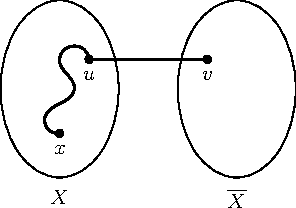
\includegraphics{path-1}
      \caption{a existência de uma aresta que ``vai''de $X$ a $\overline{X}$.}
      \label{fig:path1}
  \end{figure}
  Isso faria com que~$v$ pertencesse a~$X$ e não a~$\overline{X}$. Portanto nenhuma aresta possui uma extremidade em~$X$ e outra em~$\overline{X}$. Disso segue que~$\overline{X} = \emptyset$,
  caso contrário os conjuntos~$X,\overline{X}$ formariam uma partição de~$V_G$ em conuntos não-vazios que violariam a hipótese de que~$G$ é conexo. Portanto~$y \in X$. Daí concluímos que existe um $(x,y)$-passeio em~$G$. Como~$x$ e~$y$ foram escolhidos arbitrariamente, segue que, para todo par de vértices~$x,y \in V_G$, existe um $(x,y)$-passeio em~$G$.

  Para provar a recíproca, vamos supor que, para todo par de
  vértices~$x,y \in V_G$ existe um $(x,y)$-passeio em~$G$, e vamos
  mostrar que~$G$ é conexo. Para mostrar que~$G$ é conexo, devemos
  provar que, para toda partição de~$V_G$ em conjuntos não-vazios~$X$ e~$Y$, existe uma aresta de~$G$ com uma extremidade em~$X$ e a outra em~$Y$. Consedere então uma partição qualquer de~$V_G$ em conjuntos
  não-vazios~$X$ e~$Y$. Como~$X$ e~$Y$ são não-vazios podemos tomar~$x
  \in X$ e~$y \in Y$.  Por hipótese, existe um $(x,y)$-passeio de~$x$
  a~$y$. Vamos chamá-lo de~$P$ e representá-lo pela sequência~$v_0, v_1 \cdots v_k$ (note que $v_0 = x$ e $v_k = y$). Seja~$i$ o primeiro índice tal que~$v_i
  \in Y$. Observe que tal índice existe e é no máximo $k$, pois $v_k = y$ e $y \in Y$. Certamente~$i > 0$ pois $v_0 = x$ e $x \in X$. Pela escolha de~$v_i$, a aresta~$v_{i-1}v_{i}$ possui uma extremidade em~$X$ e outra em~$Y$. Como a partição~$\{X,Y\}$ é arbitrária, concluimos que toda bipartição de $V_G$ possui uma aresta que ``cruza'' suas partes e, portanto, $G$ é conexo.
\end{proof}

\begin{exer}
Use a Proposição~\ref{conex_prop} para mostrar que um grafo~$G$ é conexo se e somente se existe um vértice~$u \in V_G$ tal que para todo $v \in V_G$ existe um $(u,v)$-passeio em~$G$.
\end{exer}

\begin{prop}
  Para todo grafo, ele ou seu complemento são conexos.
\end{prop}

\begin{proof} 
Seja~$G = (V,E)$ um grafo qualquer. Se~$G$ é conexo, não há nada a ser demonstrado. Suponha então que~$G$ seja desconexo. Lembre-se de que o complemento de $G$ possui o mesmo conjunto~$V$ de vértices. Pela definição de grafo desconexo, existe uma partição de~$V$ em conjuntos não-vazios~$X,Y$ em que toda aresta de~$G$ está ou contida em~$X$ ou contida em~$Y$ (i.e. nenhuma aresta cruza $\{X, Y\}$). Em~$\overline{G}$, portanto, toda aresta que liga um vértice de~$X$ a um vértice de~$Y$ deve estar presente. Usando esse fato, é fácil verificar que para todo par de vértices~$u,v \in V$ existe um $(u,v)$-passeio em~$\overline{G}$. O resultado desejado segue, então, por uma aplicação da Proposição~\ref{conex_prop} ao grafo~$\overline{G}$.
\end{proof}


\begin{prop}
  Todo grafo conexo com~$n$ vértices possui pelo menos~$n-1$ arestas.
\end{prop}

\begin{proof}
A prova será algorítmica. Em cada iteração temos um conjunto~$X$ de vértices marcados e um conjunto~$Y$ de não-marcados. Antes da primeira iteração, um único vértice está marcado (a escolha desse vértice é feita arbitrariamente). Enquanto ainda existirem vértices não-marcados ($Y \neq \emptyset$), faça o seguinte: escolha uma aresta~$e$ ligando um vértice de~$X$ a um vértice de~$Y$ (tal aresta deve existir pois~$G$ é conexo e $\{X,Y\}$ é uma partição de~$V_G$); considere como marcada a extremidade de~$e$ que está em~$Y$; atualize os conjuntos~$X$ e~$Y$; repita.

Note que o conjunto~$X$ dos vértices marcados aumenta de~$1$ após cada iteração. Após~$n - 1$ iterações o algoritmo pára, pois todos os vértices estarão marcados. Note também que cada aresta de~$G$ só pode ser escolhida uma única vez, pois em iterações futuras
ela possuirá ambas as extremidades marcadas e portanto estará contida em~$X$. Asim sendo, $G$ contém pelo menos~$n - 1$ arestas como queríamos demonstrar.
\end{proof}

\begin{exer}
Mostre que, se~$G$ é um grafo conexo, então existe uma ordem~$v_1, \dots, v_n$ dos vértices de~$G$ tal que, para cada $i \in \{1,\dots,n\}$, o subgrafo $G[\{v_1,\dots,v_i\}]$ %(induzido pelos $i$ primeiros vértices dessa ordem)
é conexo.
\end{exer}

Uma \emph{componente} de um grafo~$G$ é um subgrafo induzido conexo maximal de~$G$. 

\subsection {Conjuntos de caminhos e conjuntos separadores }

As notas desta seção foram baseadas na Seção 9.1 de~\cite{BondyMurty}. 

Dado um grafo~$G$ e dois vértices distintos~$x,y \in V_G$, definimos a $(x,y)$-\emph{conexidade} como sendo o número máximo de $(x,y)$-caminhos internamente disjuntos no grafo~$G$. Para que esta definição esteja completa, precisamos dizer o que significa ``internamente disjuntos''. Dado um conjunto de $(x,y)$-caminhos $Q_1, Q_2, \dots, Q_k$, dizemos que eles são \emph{internamente disjuntos} se, para todo par de índices $i \neq j$, os únicos vértices que estão em ambos~$Q_i$ e~$Q_j$ são as suas extremidades, ou seja, os vértices $x$ e~$y$. Vamos denotar a $(x,y)$-conexidade por $p(x,y)$.

\begin{exem}
No grafo completo $K_n$, quaisquer dois vértices $u,v$ estão ligados por um caminho de comprimento~1 (através da aresta $uv$) e por $n-2$ caminhos internamente disjuntos de comprimento~$2$. Portanto, para qualque par de vértices $u,v$ no $K_n$, vale $p(u,v) = n - 1$.
\end{exem}

Se $S \subseteq V_G$ é um subconjunto de vértices, $x,y \not\in S$ e não existe $(x,y)$-caminho em $G[V \setminus S]$, então chamamos $S$ de conjunto $(x,y)$-\emph{separador} em~$G$. Note que, se $xy \in E_G$, então $G$ não possui conjunto $(x,y)$-separador. Para $xy \not\in E_G$, podemos denotar o tamanho mínimo de um conjunto $(x,y)$-separador por $c(x,y)$. Se $xy \in E_G$, então não existe conjunto $(x,y)$-separador. No entanto, se $xy \in E_G$, definimos $c(x,y)$ como 
\begin{equation}
  \label{eq:c_adjacent}
   c(x,y) = 1 + c_{G - xy}(x,y). 
\end{equation}

Veremos mais adiante, o Teorema~\ref{teor:menger}, que estabelece uma relação forte entre as quantidades $p(x,y)$ e $c(x,y)$. Comecemos por observar uma desigualdade simples envolvendo esses parâmetros. 

\begin{prop} 
\label{prop:easy_ineq_menger}
Se~$G$ é um grafo qualquer e $x,y$ são vértices distintos e não adjacentes em~$G$, então
  \begin{equation}
    \label{eq:min_max_conn}
     c(x,y) \geq p(x,y).
  \end{equation}
\end{prop}

\begin{proof}
Considere um conjunto $(x,y)$-separador $S$ e considere um conjunto $\mathcal{P}$ com caminhos internamente disjuntos de~$x$ até~$y$. Se não existe $(x,y)$-caminho em $G[V \setminus S]$, então $S$ deve conter pelo menos um vértice de cada caminho em $\mathcal{P}$ e, portanto, devemos ter 
\[ |S| \geq |\mathcal{P}|. \]
Como a desigualdade acima é válida para quaisquer escolhas de $S$ e $\mathcal{P}$, segue a validade da inequação~\eqref{eq:min_max_conn}.
\end{proof}

\begin{exer}
\label{exer:min_max}
Seja $S$ um conjunto $(x,y)$-separador e seja $\mathcal{P}$ um conjunto de $(x,y)$-caminhos internamente disjuntos. Mostre que, se $|S| = |\mathcal{P}|$, então $S$ é mínimo e $\mathcal{P}$ é máximo.
\end{exer}

O Teorema~\ref{teor:menger}, conhecido como Teorema de Menger, afirma que a recíproca do Exercício~\ref{exer:min_max} é verdade. Ou seja, ele afirma que, na realidade, a desigualdade~\eqref{eq:min_max_conn} é uma igualdade.

%Talvez a prova mais simples do Teorema de Menger seja a que faz uso da teoria de fluxos em redes. Neste texto, porém, vamos reproduzir uma prova de Göring~\cite{Goring}. Para tanto, precisamos de mais uma definição. 

% \subsubsection{Contração de um conjunto de vértices}

% Seja $G$ um grafo e seja $Y \subseteq V_G$ um subconjunto não vazio de vértices. Vamos denotar a \emph{contração} de~$Y$ em~$G$ por $G/Y$, e vamos definir esse grafo $G/Y$ como sendo o grafo obtido de $G$ depois de
% \begin{enumerate}
% \item remover do grafo todas as arestas que incidem em vértices de $Y$;
% \item \label{contr:step1} escolher $y \in Y$;
% \item remover do grafo todos os vértices de $Y$, exceto o vértice $y$; 
% \item para cada aresta $xz \in E_G$ com $x \not\in Y$ e $z \in Y$, acrescentar uma aresta $xy$, se tal aresta ainda não foi acrescentada.
% \end{enumerate}
% % remoção de $Y$ (e de todas as arestas incidentes a $Y$), pelo acrescimo de um novo vértice~$y$ e, para todo $u \in V_G \setminus Y$, pelo acrescimo da aresta $uy$ se existir pelo menos uma aresta $ux \in E_G$ para algum $x \in Y$. Ou seja, $G/Y$ é o grafo
% Ou seja, $G/Y = (V,E)$ onde
% \begin{align*}
%   V &= (V_G \setminus Y) \cup \{y\}\\
%   E &= \{ uv \in E_G \colon u,v \not\in Y\} \cup \{xy \colon x \in V_G \setminus Y \text{ e } \exists\,z\in Y \text{ tal que }xz \in E_G\}.
% \end{align*}


% \begin{exem}
% No exemplo da Figura~\ref{fig:contr} abaixo, todo vértice vizinho de alguém em $Y$, depois da contração, será vizinho de $y$.
% \begin{figure}[H]
% \centering
% \begin{subfigure}{.5\textwidth}
%   \centering
%   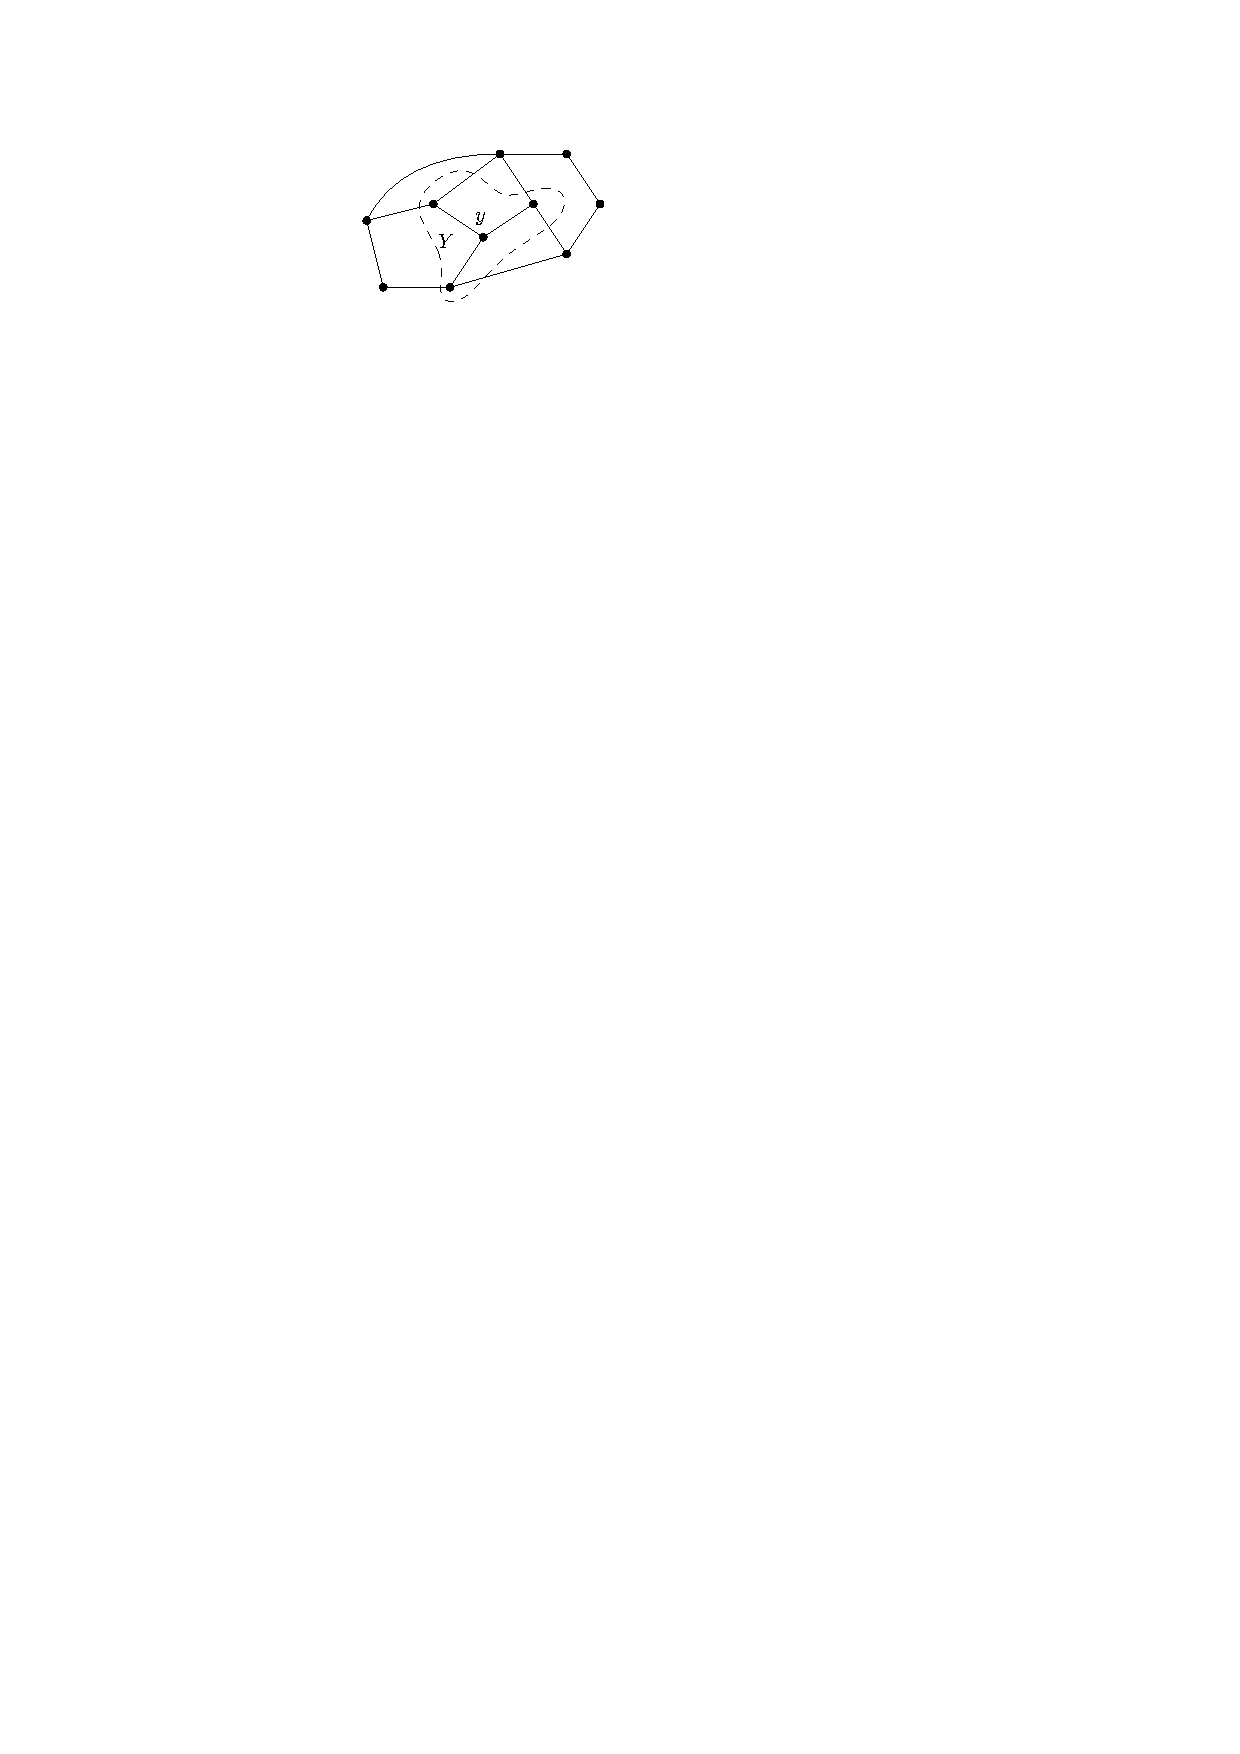
\includegraphics[]{contracao.pdf}
%   \caption{o grafo~$G$ e o conjunto $Y$.}
%   \label{fig:contr1}
% \end{subfigure}%
% \begin{subfigure}{.5\textwidth}
%   \centering
%   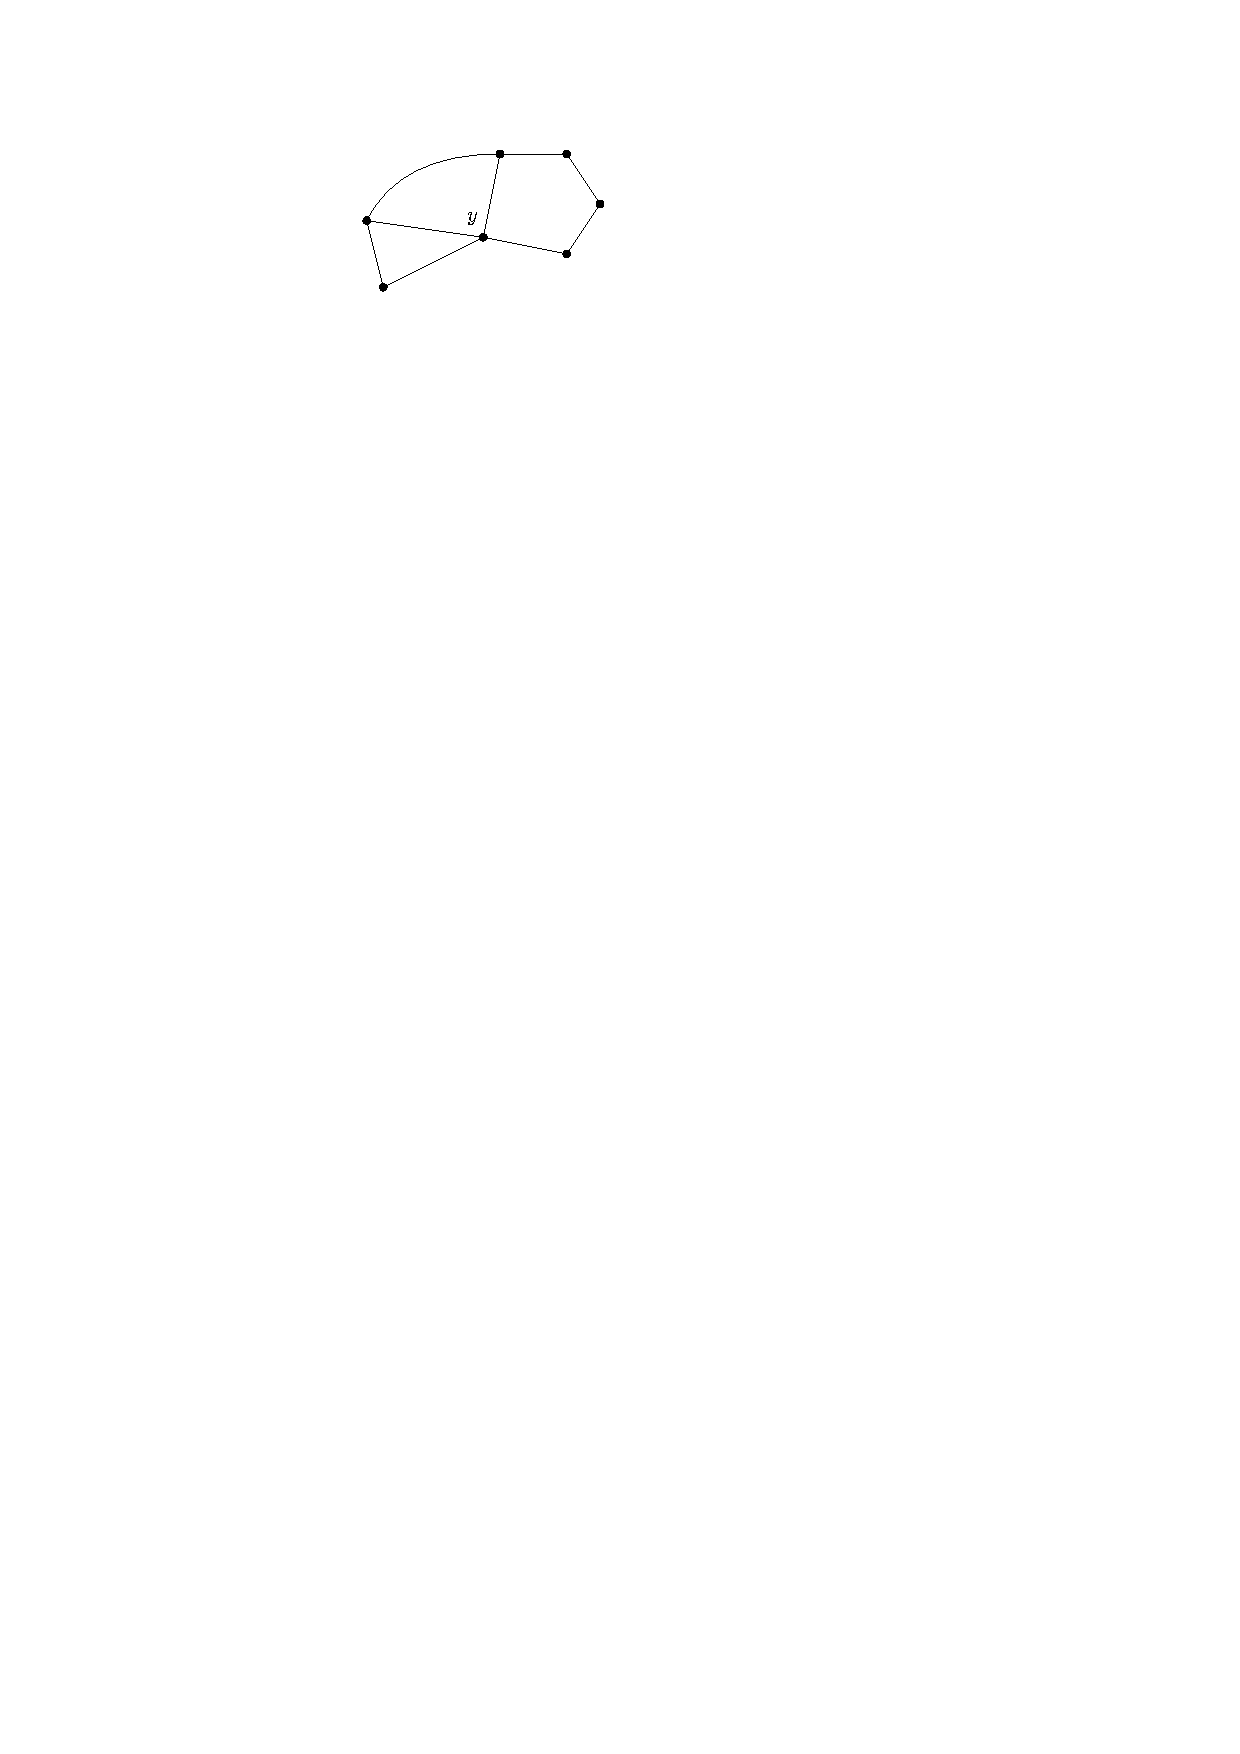
\includegraphics[]{contraido.pdf}
%   \caption{o grafo~$G/Y$.}
%   \label{fig:contr2}
% \end{subfigure}
% \caption{a contração de um conjunto $Y$ no grafo~$G$.}
% \label{fig:contr}
% \end{figure}
% \end{exem}

% \noindent Observe que a escolha do vértice $y$, no passo~\ref{contr:step1} da definição de $G/Y$, é irrelevante. 

% %Na prova do Teorema de Menger, o conjunto $Y$ que iremos contrair é um par de vértices adjacentes, i.e. uma aresta $e \in E_G$. Nesse caso, escrevemos $G/e$ para denotar o grafo contraído.

\subsubsection {Teorema de Menger}


% \begin{lema}
% \label{lema:c_contracted}
% Seja $G$ um grafo, seja $Y \subseteq V_G$ um subconjunto de vértices e, para um vértice $y \in Y$, seja $G/Y$ o grafo obtido contraindo-se o conjunto $Y$ ao vértice $y$. Se $x \in V_G \setminus Y$, então $c_{G/Y}(x,y) \geq c_G(x,y)$.
% \end{lema}

% \begin{proof}
%   Seja $S$ um conjunto $(x,y)$-separador em $G/Y$. Suponha, com a finalidade de chegarmos a uma contradição, que $S$ não seja um conjunto $(x,y)$-separador em $G$. Nesse caso, $G - S$ possui um $(x,y)$-caminho $v_0 v_1 \cdots v_k$ (e, portanto, $v_0 = x$ e $v_k = y$). Seja $i > 0$ o menor índice tal que $v_i \in Y$. Observe que tal índice existe e satisfaz $i \leq k$, pois $v_k = y$ e $y \in Y$. Assim, o caminho $v_0 v_1 \cdots v_{i-1} y$ é um $(x,y)$-caminho em $G/Y$ que evita $S$: uma contradição com a propriedade de que $S$ é $(x,y)$-separador em $G/Y$. 

% Podemos supor, então, que todo conjunto $(x,y)$-separador em $G/Y$ é também $(x,y)$-separador em $G$. Portanto, é verdadeira a desigualdade almejada no enunciado.
% \end{proof}

% \begin{lema}
% \label{lema:all_paths_size_2}
% Seja $G$ um grafo e sejam $x,y \in V_G$ dois vértices distintos. Seja $\mathcal{P}$ uma coleção máxima de $(x,y)$-caminhos internamente disjuntos em~$G$ e seja $S$ o conjunto de vértices que estão em algum $(x,y)$-caminho de~$\mathcal{P}$. Se todo vértice $s \in S$ é adjacente a ambos~$x$ e~$y$, então $p(x,y) = c(x,y)$.
% \end{lema}

% \begin{proof}
% Note que $S$ é um conjunto $(x,y)$-separador em~$G$. Seja $\mathcal{Q}$ a coleção de $(x,y)$-caminhos internamente disjuntos definida por
% \[ \mathcal{Q} = \{xsy \colon s \in S\}. \]
% Note que $|S| = |\mathcal{Q}|$. Pelo Exercício~\ref{exer:min_max}, temos que $c(x,y) = p(x,y)$.
% \end{proof}


\begin{teor}
\label{teor:menger}
Se~$G$ é um grafo de ordem $n \geq 2$ e $x,y$ são vértices distintos em~$G$, então
\begin{equation}
  \label{eq:min_max_conn2}
  c(x,y) = p(x,y).
\end{equation}
\end{teor}

\begin{proof}
  A prova é por indução em~$m$. Para estabelecermos a base da indução, devemos provar que o teorema vale para todo o grafo vazio com $n \geq 2$ vértices. De fato, em qualquer grafo vazio~$E_n$, se tomarmos dois vértices $x \neq y$, não há caminho de $x$ a~$y$ e, portanto, $p(x,y) = c(x,y) = 0$.

Para provarmos o passo de indução, seja $G$ um grafo qualquer com $m > 0$ arestas, e sejam $x,y$ dois vértices distintos de~$G$. Suponha que qualquer grafo com menos que $m$ arestas satisfaz~\eqref{eq:min_max_conn2}. Se $xy \in E_G$, então aplicamos a hipótese de indução em $G - xy$ e facilmente obtemos que $G$ deve satisfazer~\eqref{eq:min_max_conn2}. Suponha, então, que $xy \not\in E_G$. Também podemos supor que $x$ e $y$ estão ligados por um caminho, do contrário $p(x,y) = c(x,y) = 0$. Além disso, podemos supor que todo vértice de $G$ está em algum $(x,y)$-caminho, pois vértices em outras componentes não influenciam nos parêmetros $p$ e $c$. 

Seja $\mathcal{P}$ uma coleção máxima de $(x,y)$-caminhos internamente disjuntos em~$G$, ou seja, $|\mathcal{P}| = p(x,y)$. 

Primeiramente supomos que existe um vértice $v \neq x,y$ que não pertence a nenhum caminho em $\mathcal{P}$. Seja $N = N_G(v)$ o conjunto de vizinhos de $v$, e considere o grafo $H$ construído da seguinte maneira:
\begin{enumerate}[(i)]
\item escolha um vizinho $u \in N$, arbitrariamente;
\item remova todas as arestas de $vw$ com $w \in N$;
\item \label{step:new_edges} para cada $w \in N - u$, acrescente a aresta $uw$, se necessário.
  \begin{figure}[H]
    \centering
    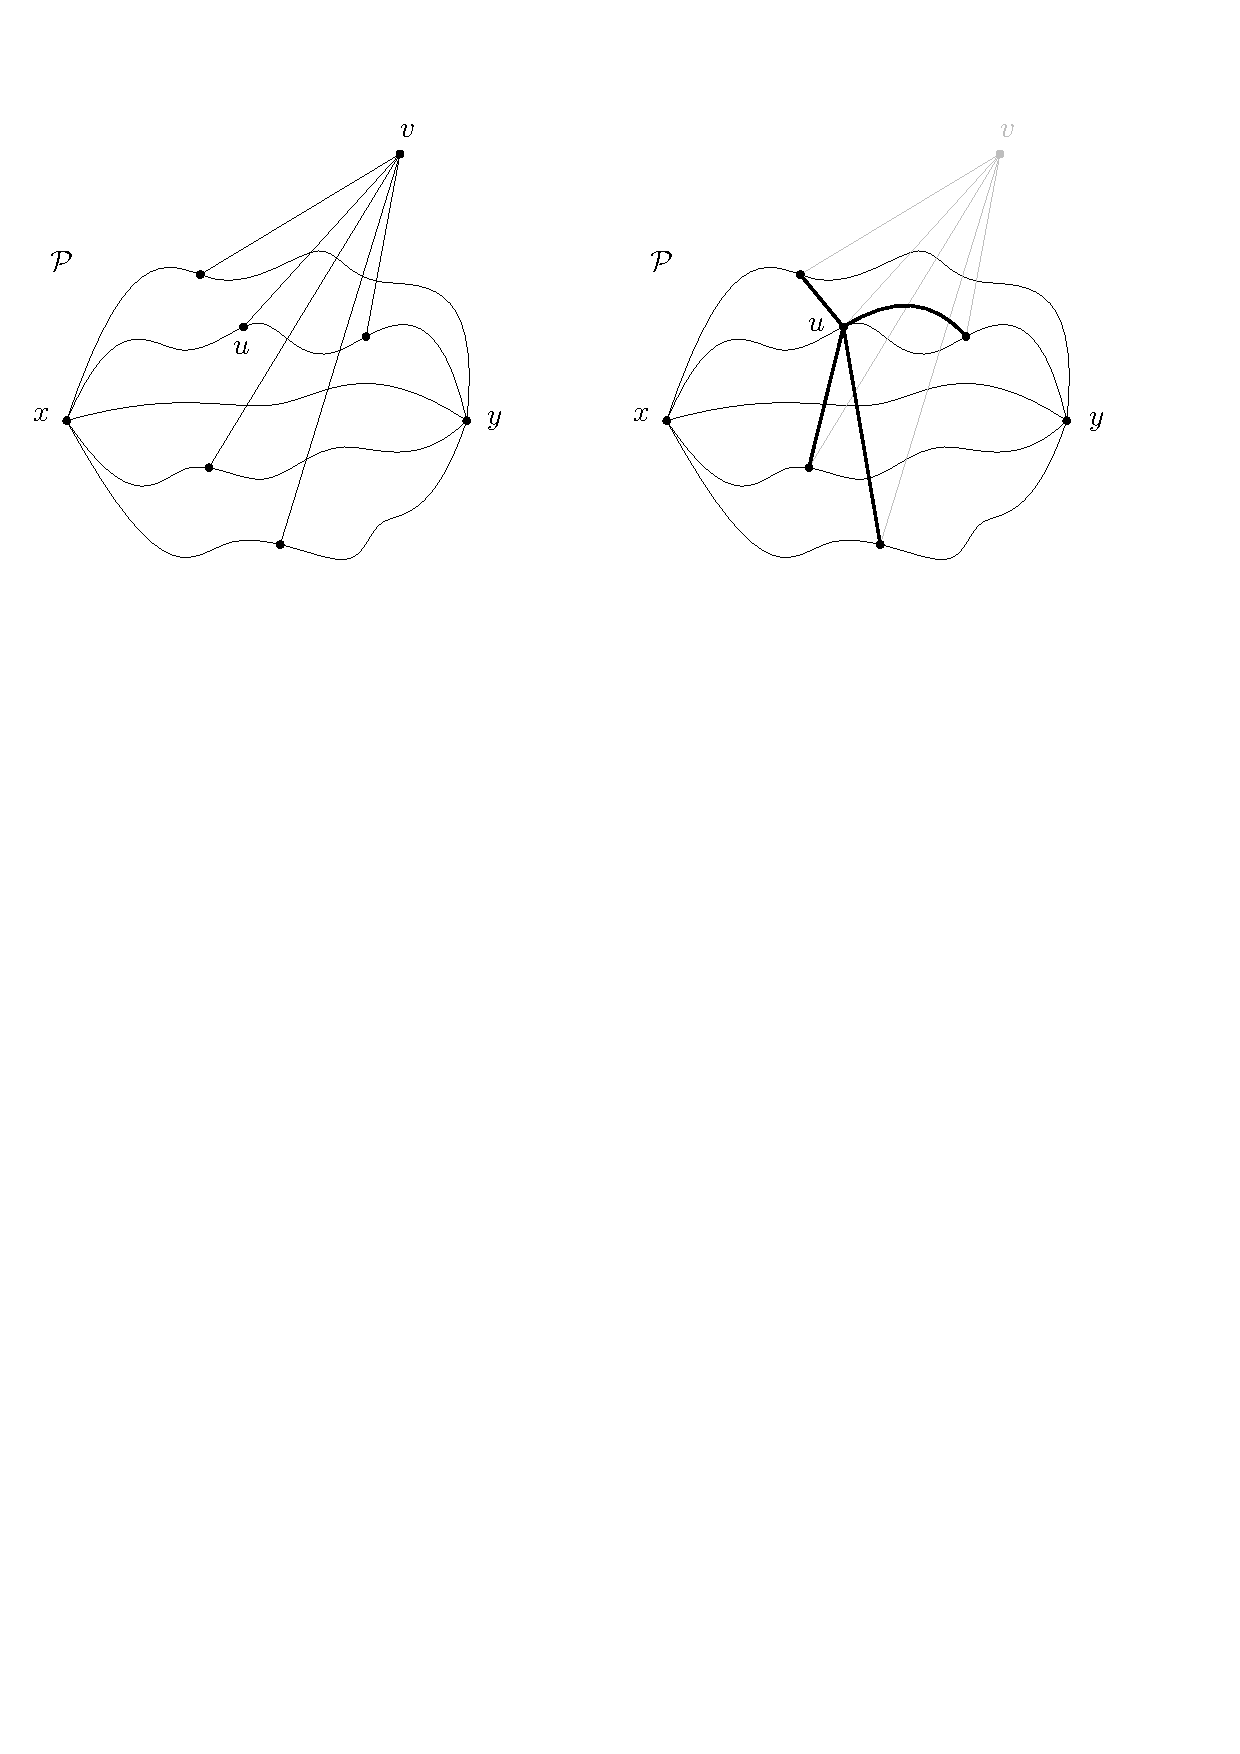
\includegraphics[scale=0.6]{grafo_H.pdf}
    \caption{construção do grafo $H$ a partir de $G$.}
    \label{fig:H_contruction}
  \end{figure}

\end{enumerate}
Para facilitar a escrita, vamos usar $c,c',p,p'$ para denotar as quantidades
\begin{align*}
  c &= c_G(x,y),\\
  c' &= c_H(x,y),\\
  p &= p_G(x,y),\\
  p' &= p_H(x,y).
\end{align*}
Note que $\mathcal{P}$ é uma coleção de $(x,y)$-caminhos internamente disjuntos em $H$, portanto $p \leq p'$. Vamos argumentar que $p \geq p'$. Suponha o contrário, e considere uma coleção $\mathcal{Q}$ de $(x,y)$-caminhos internamente disjuntos em $H$ com $|\mathcal{Q}| > p$. Note que $\mathcal{Q}$ não pode ser uma coleção de $(x,y)$-caminhos internamente disjuntos em $G$. Portanto, o vértice $u$ deve estar em algum $(x,y)$-caminhos $Q \in \mathcal{Q}$ e, além disso, uma ou duas arestas acrescentadas no passo~\eqref{step:new_edges} devem ser percorridas por $Q$. Em ambos os casos, seria possível usar o vértice~$v$ no grafo $G$ para construir uma coleção de caminhos $\mathcal{Q}'$ com mais do que $p(x,y)$ caminhos: uma contradição.
\begin{figure}[H]
  \centering
  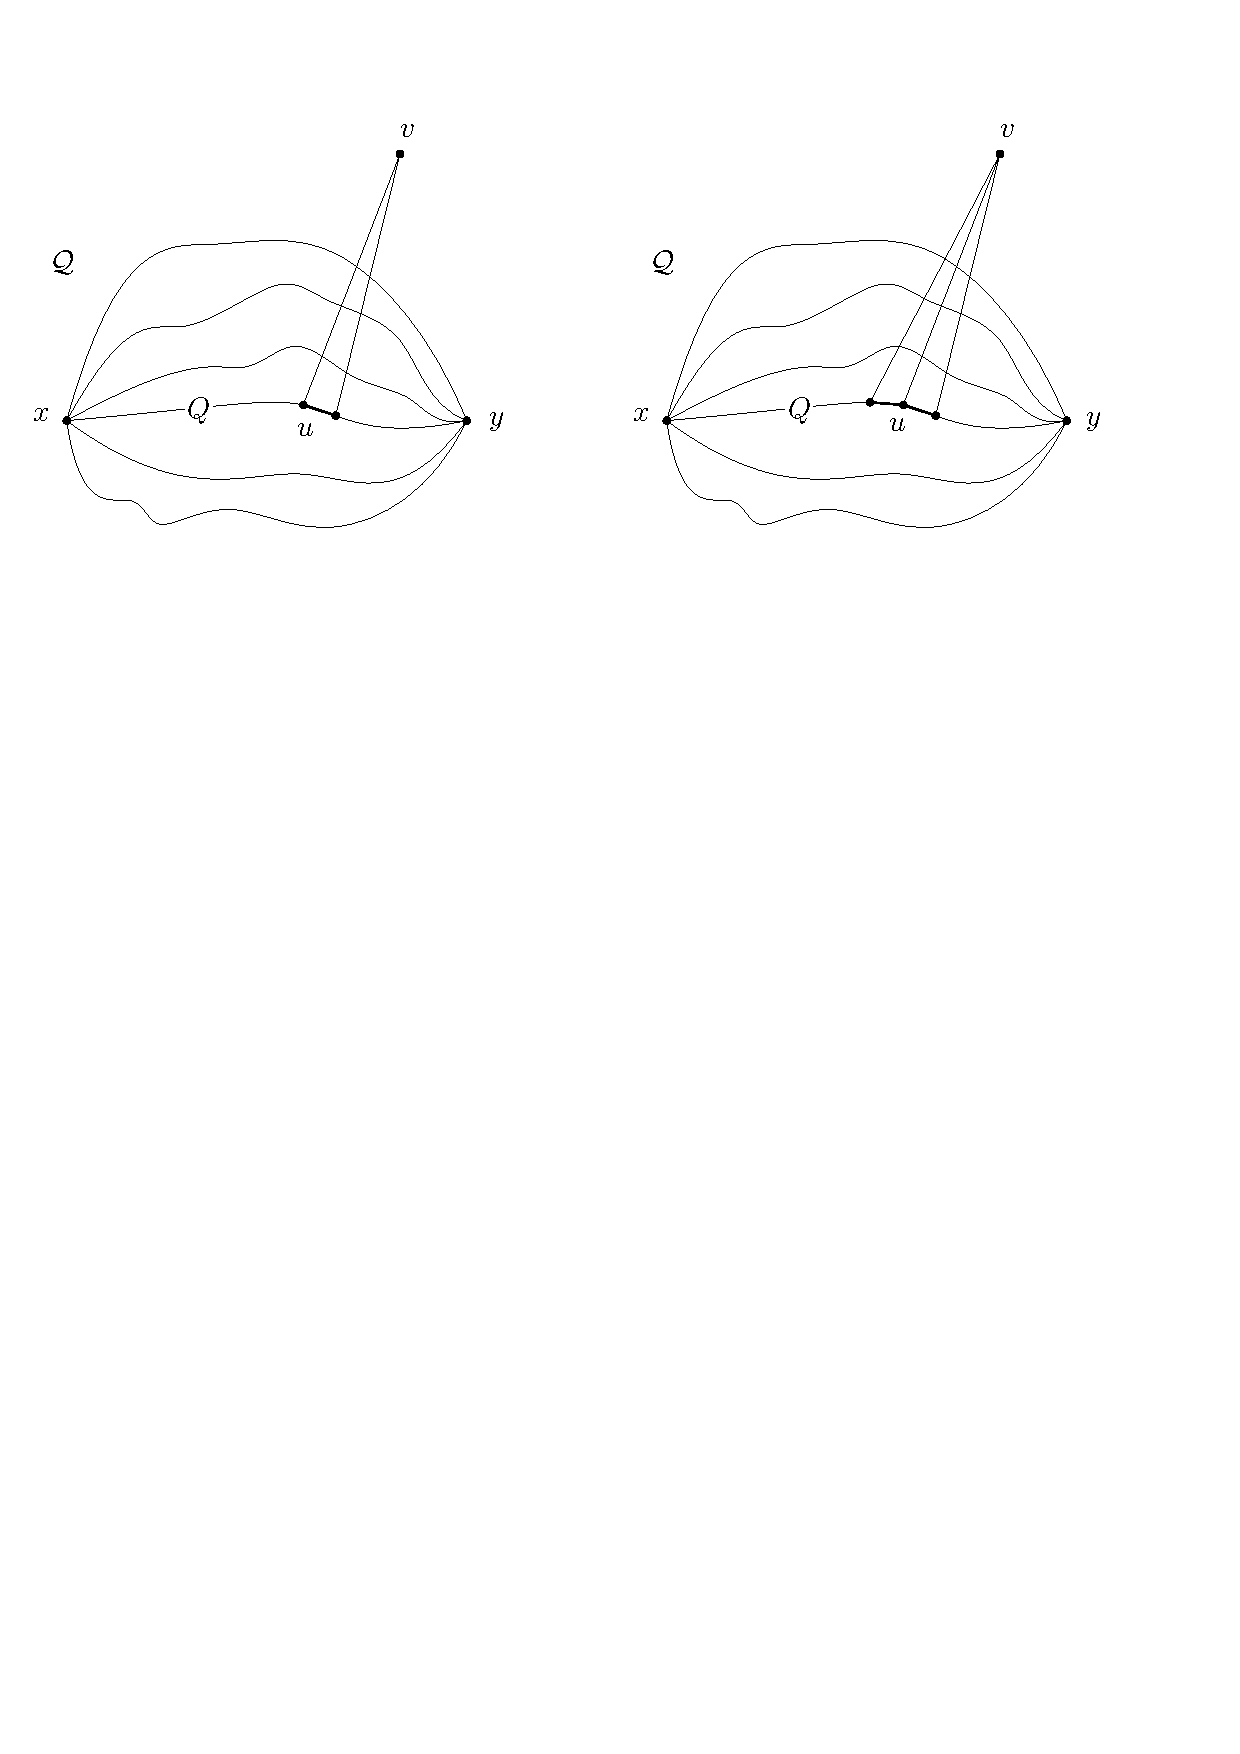
\includegraphics[scale=0.6]{caminhos_Q.pdf}
  \caption{usando $\mathcal{Q}$ e $v$ para construir uma coleção de caminhos em~$G$.}
  \label{fig:bigger_collection}
\end{figure}
Portanto $p = p'$. 

Observe também que todo conjunto $(x,y)$-separador em $H$ é também $(x,y)$-separador em $G$. Portanto $c \leq c'$. Aplicando a hipótese de indução no grafo $H$, temos que $c' = p'$. Juntando a esses fatos a desigualdade~\eqref{eq:min_max_conn} da Proposição~\ref{prop:easy_ineq_menger}, temos que 
\[ c \leq c' = p' = p \leq c, \]
Portanto $c = p$ como gostaríamos.
Sendo assim, podemos supor que toda coleção máxima de $(x,y)$-caminhos internamente disjuntos em~$G$ usa todos os vértices de $G$, o que significa que $N(x)$ é um conjunto $(x,y)$-separador com $p(x,y)$ vértices, o que implica, pelo Exercício~\ref{exer:min_max}, que $c(x,y) = p(x,y)$.

Pelo princípio de indução finita, segue a validade do teorema.
\end{proof}


Enunciar a versão do teorema de menger para caminhos aresta disjuntos


Explicar o que é multigrafo

Falar do Fan Lemma 








\section{Mais exemplos de grafos}

$\rhd$ O hipercubo $Q_k$\\
$\rhd$ O grafo de Petersen\\
$\rhd$ O grafo bipartido completo $K_{s,t}$


\section {Grafos bipartidos}

Um grafo $G$ é \emph{bipartido} se $V_G$ pode ser escrito como união de conjuntos disjuntos $X \cup Y$ de forma que toda aresta de $G$ possui uma extremidade em $X$ e outra em $Y$. Observe que não necessáriamente $\{X,Y\}$ é uma partição de~$V_G$, pois $X$ ou $Y$ pode ser vazio no caso de $G$ não ter arestas.

\begin{exem}
O caminho $P_n$ é um grafo bipartido. A estrela $S_{n-1}$ também. $K_2$ é bipartido mas $K_3$ não é bipartido. $C_4$ é bipartido, mas $C_3$ não.
\end{exem}

\begin{exer}
Mostre que qualquer hipercubo $Q_k$ é bipartido. 
\end{exer}

\begin{exer}
Mostre que qualquer grade $G_{s \times t}$ é bipartido.
\end{exer}

%% B&M 1.1.2 (b)
\begin{exer}
Mostre que todo grafo bipartido satisfaz $m \leq n^2/4$.
\end{exer}

\begin{exer}
\label{exer:cimpar}
Mostre diretamente que qualquer circuito ímpar $C_{2k+1}$ não é um grafo bipartido.
\end{exer}

\begin{exer}
\label{exer:uni_bip}
Mostre que união disjunta de grafos bipartidos é um grafo bipartido.
\end{exer}

\begin{prop}
Um grafo $G$ é bipartido se e somente se $G$ não possui um circuito ímpar. 
\end{prop}

\begin{proof}
O Exercício~\ref{exer:cimpar} acima estabelece uma das direções da proposição. Resta mostrar a direção recíproca. Mais especificamente, resta mostrar que um grafo que não possui um circuito ímpar é bipartido. 
Note também que, pelo Exercício~\ref{exer:uni_bip}, se cada componente conexa de~$G$ for um grafo bipartido, então~$G$ é bipartido.
\end{proof}

\bibliographystyle{plain}
\bibliography{main.bib}
\end{document}
